\chapter{COULOMB'S LAW AND ELECTRIC FIELD}



In electrostatics we deal with the properties and phenomenon associated with charges that are not in motion. Let's start with electric charges.
\section{Charge}
\begin{definition}
	The physical quantity charge is a basic property of matter, carried by some elementary particles. This governs how the particles are affected by an electric or magnetic field .There  are  two  types  of  observed  electric  charges,  which  we  designate  as  positive  and  negative.
\end{definition}
\subsubsection{Properties of Electric charge}
\begin{itemize}
	\item Charge is quantized $Q=ne$ where, $ n=0,\pm1,\pm2,\pm3 \cdots$
	\item In the SI system, the basic unit of charge is coulomb (C)
	\item  The smallest unit of `free' charge known in nature is the charge of an electron or proton. The charge of a single electron, $-e$, is $-1.60 \times 10^{-19} \mathrm{C}$, and the charge of a single proton, $+e$, is $+1.60 \times 10^{-19} \mathrm{C} .$
	\item Charges obey additive property.
	\item In a closed system , the total amount of charge is conserved since charge can neither be created nor be destroyed. And a charge can be transferred from one body to another.
\end{itemize}
\subsection{Continous Charge Distributions}
\bigskip
\subsubsection{Linear Charge Distribution}
If the charge is spread out along a line , with charge per unit length $\lambda$, it is called the \textbf{linear charge distribution.}\\
\begin{minipage}{0.45\textwidth}
	\begin{align*}
	\lambda&=\frac{dq}{d l}\\
	\Longrightarrow d q&=\lambda d l \ \text { or }\ q=\int \lambda d l\\
	\end{align*}
\end{minipage}\hfil
\begin{minipage}{0.45\textwidth}
	\begin{figure}[H]
		\centering
		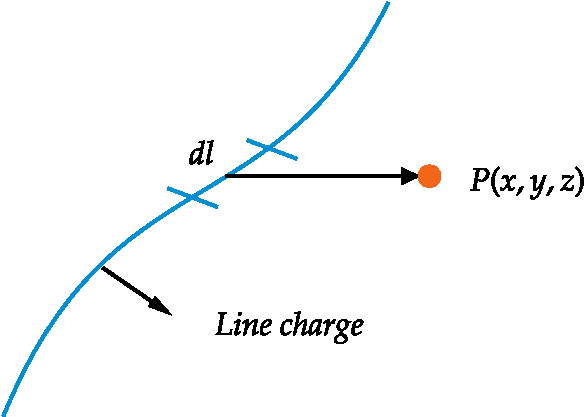
\includegraphics[height=3.5cm,width=5cm]{linear charge}
		\caption{Linear charge distribution}
		\label{linear}
	\end{figure}
\end{minipage}

\subsubsection{Surface Charge Distribution}
If the charge is smeared out over a surface , with charge per unit area $\sigma$, it is called the \textbf{surface charge distribution.}\newline
\begin{minipage}{0.45\textwidth}
\begin{align*}
\sigma&=\frac{dq}{d s}\\
\Longrightarrow d q&=\sigma d s\ \text { or }\ q=\int \sigma d s\\
\end{align*}
\end{minipage}\hfill
\begin{minipage}{0.45\textwidth}
	\begin{figure}[H]
		\centering
		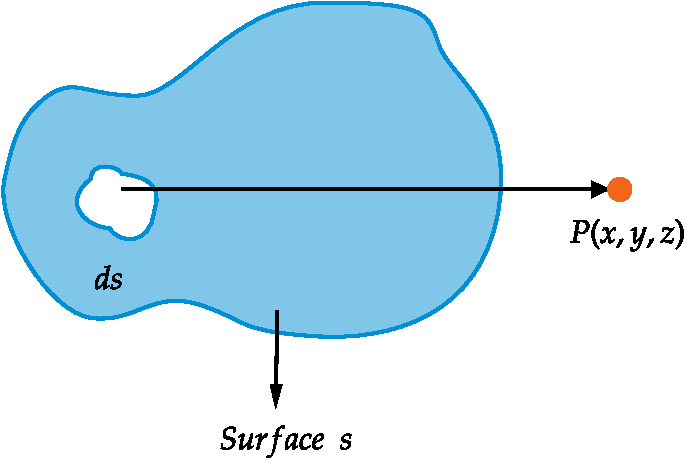
\includegraphics[height=3.5cm,width=5cm]{surface}
		\caption{Surface charge distribution}
		\label{rc current discharge}
	\end{figure}
	
\end{minipage}

\subsubsection{Volume Charge Distribution}
If the charge fills a volume , with charge per unit volume $\rho$, it is called the \textbf{volume charge distribution.}
\begin{minipage}{0.45\textwidth}
	\begin{align*}
	\rho&=\frac{dq}{d v}\\
	\Longrightarrow d q&=\rho d v\ \text { or } \ q=\int \rho d v\\
	\end{align*}
\end{minipage}\hspace{2cm}
\begin{minipage}{0.45\textwidth}
		\begin{figure}[H]
		\centering
		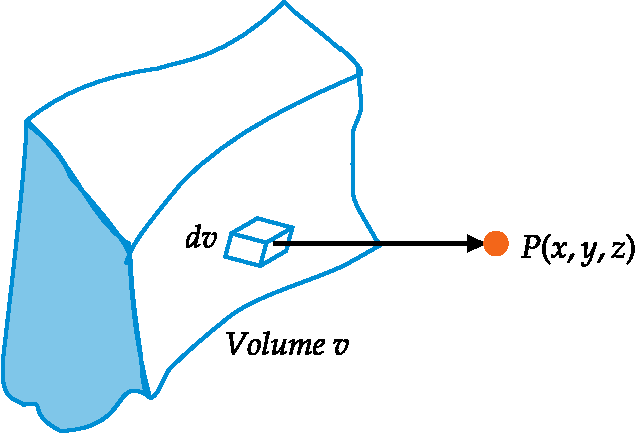
\includegraphics[height=3.5cm,width=5cm]{volume}
		\caption{Volume charge distribution}
		\label{volume}
	\end{figure}
\end{minipage}

\subsection{Coulomb's Law}
\begin{definition}
The electric force on a test charge `$Q$' due to a single point charge `$q$' at rest , with respect to each other,  at a distance `$r$' is proportional to the product of the two charges  ($Qq$ ) and is inversely proportional to the square of the seperation distance ($r^{2}$)  between them.
\begin{equation}
 F={\frac{1}{4\pi \epsilon_{0}}} \frac{Qq}{r^{2}}\hat{r}
\end{equation}
Where  $\hat{{r}}=\frac{\vec{r}}{r}$ is a unit vector from the location of $ q $ to  the location of $ Q $.
\end{definition}
The constant $\epsilon_{0}$ is called the permitivity of free space. In SI units, where force is in Newtons (N), distance in meters (m), and charge in coulombs (C). Coulomb's conclusions apply to charges in vaccum or in media of negligible susceptibility.
$$
\epsilon_{0}=8.85 \times 10^{-12} \frac{\mathrm{C}^{2}}{\mathrm{~N} \cdot \mathrm{m}^{2}}
$$
The electrostatic force with which we are concerned with is less than $1 \%$ of the strong nuclear force.
\subsubsection{Vector Form}
Let $\vec{r}_{1}$ and $\vec{r}_{2}$ are position of two charges $q_{1}$ and $q_{2}$.
	\begin{figure}[H]
	\begin{center}
		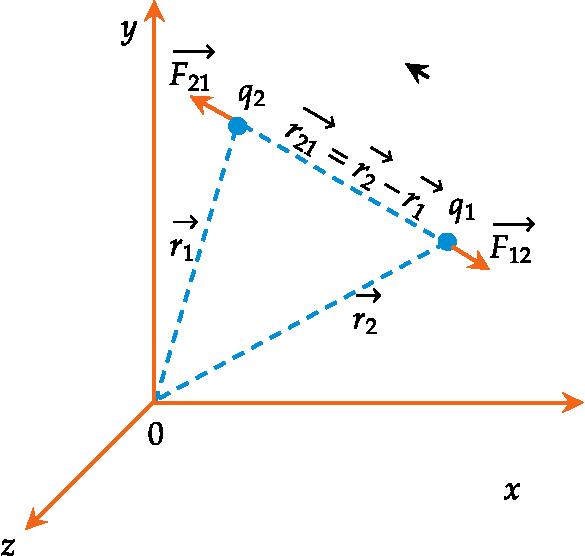
\includegraphics[width=0.30\textwidth]{coulombs law}
	\end{center}
	\caption{Coulomb's law}
\end{figure}
\begin{align}
\intertext{According to Coulomb law the force on $q_{2}$ due to $q_{1}$ is}
\vec{F}_{21}&=\frac{1}{4 \pi \varepsilon_{0}} \frac{q_{1} q_{2}}{r_{21}^{2}} \hat{r_{21}}=\frac{1}{4 \pi \varepsilon_{0}} \frac{q_{1} q_{2}}{r_{21}^{3}} \vec{r}_{21}\label{coulombs1}\\
\intertext{The force on $q_{1}$ due to $q_{2}$ is}
\vec{F}_{12}&=\frac{1}{4 \pi \varepsilon_{0}} \frac{q_{1} q_{2}}{r_{12}^{2}} \hat{r}_{12}=-\frac{1}{4 \pi \varepsilon_{0}} \frac{q_{1} q_{2}}{r_{21}^{2}} \hat{r}_{21} \label{coulombs2}
\intertext{And then from \ref{coulombs1} and \ref{coulombs2} we get,}
\vec{F}_{21}&=-\vec{F}_{12}
\end{align}
This is a confirmation of Newton's third law,that the force on the charge $q_{1}$ due to $q_{2}$ is equal and opposite to that of   $q_{2}$ due to $q_{1}$. 
\subsection{Principle of Superposition }
Coulomb’s  law  applies  to  any  pair  of stationary  point  charges.  When  more  than  two  charges  are  present, the net force on any one charge is simply the vector sum of the forces exerted on it  by  the  other  charges. 
If we have several point charges $q_{1}, q_{2}, \ldots, q_{n}$, at distances $r_{1}, r_{2}, \ldots, r_{n}$ from $Q$, the total force on $Q$ is ,
\begin{align}
\vec{F} &=\vec{F}_{1}+\vec{F}_{2}+\ldots=\sum\vec{F_{n}} \\
&=\frac{1}{4 \pi \epsilon_{0}}\left(\frac{q_{1} Q}{r_{1}^{2}} \hat{\boldsymbol{r}}_{1}+\frac{q_{2} Q}{r_{2}^{2}} \hat{\boldsymbol{r}}_{2}+\ldots\right) \notag\\
&=\frac{Q}{4 \pi \epsilon_{0}}\left(\frac{q_{1} \hat{\boldsymbol{r}}_{1}}{r_{1}^{2}}+\frac{q_{2} \hat{\boldsymbol{r}}_{2}}{r_{2}^{2}}+\frac{q_{3} \hat{\boldsymbol{r}}_{3}}{r_{3}^{2}}+\ldots\right)\notag
\end{align}
This is called the principle of superposition.
\newline \newline For a system of $n$ charges, the net force experienced by the $j$ th particle would be,
\begin{align*}
{\vec{F}}_{j}&=\sum_{i=1 \atop i \neq j}^{n} \vec{{F}}_{i j}
\intertext{Where $\vec{{F}}_{i j}$ denotes the force between particles $i$ and $j .$}
\end{align*}
 The superposition principle implies that the net force between any two charges is independent of the presence of other charges.(This is true if the charges are in fixed positions.) 
\begin{exercise}
	Consider two positive charges of magnitude $q$ seperated by a distance$d$ .A third charge $+Q$ is situauted as shown in the figure calculate the total force on $+Q$
	\begin{center}
	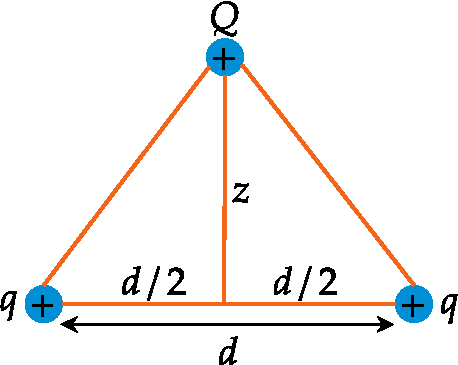
\includegraphics[width=0.30\textwidth]{p-1 coulombs}
	\end{center}
	\end{exercise}
\begin{answer}
	{According to superposition principle,The force on $+Q$ is,}\newline
	\begin{minipage}{0.65\textwidth}
		\begin{align*}
	F_{total}&=F_{1}+F_{2}\\
	\intertext{Here,} F_{1}&=F_{2}=F=\frac{1}{4 \pi \epsilon_{0}}\frac{Qq}{(z^{2}+d^{2}/4)}
	\intertext{Since $\quad |F_{1}|=|F_{2}| $\  their x-component cancells out.}
	\intertext{Then,}
	F_{total}&=F_{1}\cos\theta \hat{j}+F_{2}\cos\theta \hat{j}\\
	F_{total}&=F\cos\theta \hat{j}+F\cos\theta \hat{j}\\
	&=2F\cos\theta \hat{j}\\
	&=2 \frac{1}{4 \pi \epsilon_{0}}\frac{Qq}{(z^{2}+d^{2}/4)} \cos\theta \hat{j}
	\intertext{But here,}\cos\theta&=\frac{z}{\sqrt {(z^{2}+d^{2}/4)}}
	\intertext{Then,}
	F_{total}&=2 \frac{1}{4 \pi \epsilon_{0}}\frac{Qq}{(z^{2}+d^{2}/4)}\frac{z}{\sqrt {(z^{2}+d^{2}/4)}}\hat{j}\\
	&= \frac{2}{4 \pi \epsilon_{0}}\frac{Qqz}{(z^{2}+d^{2}/4)^{3/2}}\hat{j}
	\end{align*}
	\end{minipage}
\begin{minipage}{0.35\textwidth}
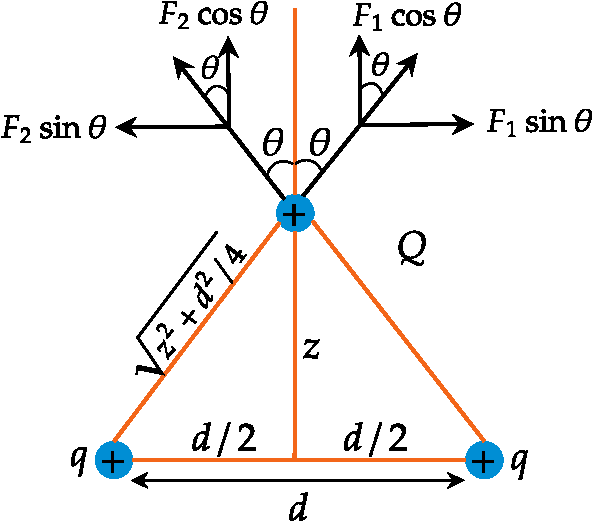
\includegraphics[width=5cm]{p-1 coulombs answer}
\end{minipage}
\end{answer}


\begin{exercise}
	Consider a thin rod of length $\ell$ and charge $Q$ apoint charge $q $ is situated at a distance $ d$  from one end of the road. Find the force between the rod and charge $q $
	\begin{figure}[H]
		\begin{center}
			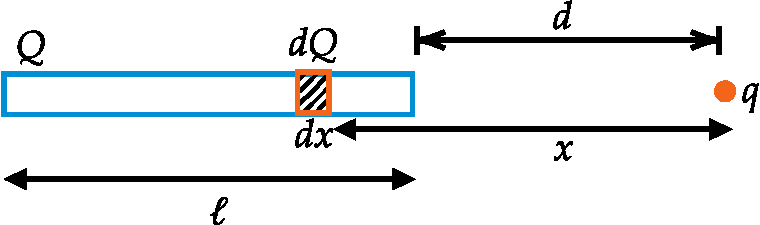
\includegraphics[width=0.35\textwidth]{coulombs p2}
		\end{center}
	\end{figure}
\end{exercise}
\begin{answer}
	\begin{align*}
	\intertext{Here, the elementary force,} dF&=\frac{1}{4\pi\epsilon_{0}}\frac{q dQ}{x^{2}}
	\intertext{But,} dQ&=\lambda dx\quad \rightarrow \lambda=\frac{Q}{\ell}
	\intertext{Then,}F&= \frac{1}{4\pi\epsilon_{0}} q\lambda \int_{d}^{d+\ell} \frac{dx}{x^{2}}\\&=\frac{1}{4\pi\epsilon_{0}} \frac{qQ}{\ell}\left[-\frac{1}{x} \right]_{d}^{d+\ell} \\&=\frac{1}{4\pi\epsilon_{0}} \frac{qQ}{\ell}\left[\frac{\ell}{(\ell+d)d}\right]\\
	&=\frac{1}{4\pi\epsilon_{0}} \frac{qQ}{(\ell+d)d}
	\end{align*}
\end{answer}
\subsection{Electric Field \textbf{$ \vec{E}$}}
The electrostatic force, like the gravitational force, is a force that acts at a distance, even
when the objects are not in contact with one another. To justify such the notion we rationalize action at a distance by saying that one charge creates a field which in turn acts on the other charge.\\\\
\textbf{Physically Electric field, $E(r)$ is the force per unit charge that would be excerted on a test charge.}
\begin{itemize}
	\item The electric field $ \vec{E}$ is a vector quantity with magnitude directly proportional to force and with direction given by the direction of the force on a positive test charge.
	\item The force that acts on the unit charge at a particular point is called electric field intensity $(\vec{E})$ at that point.
	\item $\vec{E}$ has a unit of $N/C$ or $V/m$.
\end{itemize}
 Consider a "test charge" $Q$ on which this charge
$ q $ exerts a force. It is necessary that $Q$ is taken infinitesimally small. This is because, $Q$ itself being an electric charge will have its own electric field which will alter the field due to the charge $ q $.  We define the electric field due to the charge $ q $ as,
\begin{align}
\notag \vec{E}&=\frac{1}{4 \pi \varepsilon_{0}}  \frac{q}{r^{2}} \hat{r}\\
\intertext{For a system of $n$ charges,}
\vec{E}&=\frac{1}{4 \pi \varepsilon_{0}} \sum_{i=1}^{n} \frac{q_{i}}{r_{i}^{2}} \hat{r}_{i}\\
\intertext{If $\vec{F}$ be force on charge $q$ due to some other charge then field at location of $q$ due to other charge is,}
\vec{F}&=q\vec{E}
\end{align}
\begin{minipage}{0.65\textwidth}
	\begin{align*}
\intertext{For continuous charge distribution,}
\vec{E}({r})&=\frac{1}{4 \pi \epsilon_{0}} \int_{{l}} \frac{\lambda\left(\mathbf{r}\right)}{r^{2}} \hat{{r}} d l\quad\rightarrow \text{Linear charge distribution}\\
\vec{E}({r})&=\frac{1}{4 \pi \epsilon_{0}} \int_{{S}} \frac{\sigma\left(\mathbf{r}\right)}{r^{2}} \hat{{r}} d a\quad\rightarrow \text{Surface charge distribution}\\	
\vec{E}({r})&=\frac{1}{4 \pi \epsilon_{0}} \int_{{V}} \frac{\rho\left({r}\right)}{r^{2}} \hat{r} d \tau\quad \rightarrow \text{Volume charge distribution}
	\end{align*}
\end{minipage}
\begin{minipage}{0.35\textwidth}\hfil
	
\begin{figure}[H]
	\begin{center}
		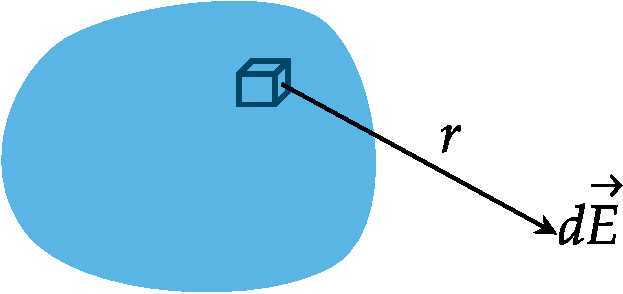
\includegraphics[width=0.85\textwidth]{Electric field}
	\end{center}
\caption{Electric field}
\end{figure}
\end{minipage}


\begin{exercise}
Consider two charges of magnitude $+q$ and  $-q$ seperated by a distance\ $2d$ .
 Find the electric field produced by these charges at a point $p$ above middle of the charges as shown in the figure.
 	\begin{center}
 		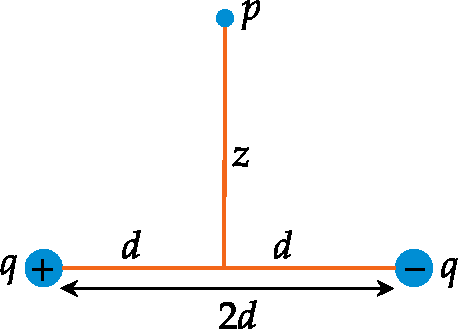
\includegraphics[width=0.25\textwidth]{electricfield p1}
 	\end{center}
 \end{exercise}
\opencutright
\renewcommand\windowpagestuff{
	\centering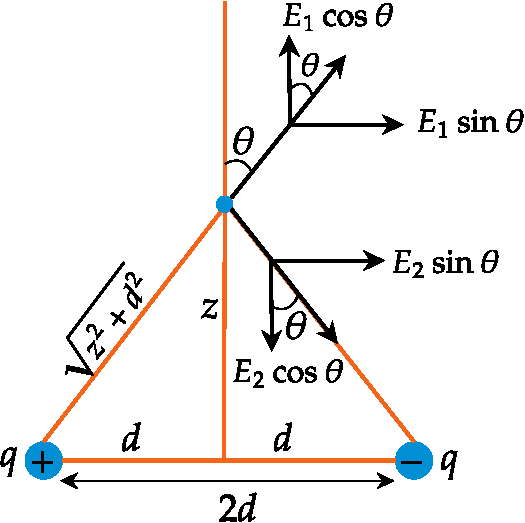
\includegraphics[width=5cm]{electricfield p1 ans}}
\begin{answer}
	\begin{cutout}{3}{\dimexpr\linewidth-4.9cm\relax}{2pt}{8}
		\begin{align*}
		\text{The Electric field at the point p is,}\\
		E_{total}&=E_{1}+E_{2}\\
		\text{Here,}\quad E_{1}&=E_{2}=E=\frac{1}{4 \pi \epsilon_{0}}\frac{q}{(z^{2}+d^{2})}\\
		\text{since }\quad |E_{1}|=|E_{2}| &\quad\text{their y-component cancells out.}\\
		\text{Then,}\\
	E_{total}&=E_{1}\sin\theta \hat{i}+E_{2}\sin\theta \hat{i}\\
		E_{total}&=E\sin\theta \hat{i}+F\sin\theta \hat{i}\\
		&=2E\sin\theta \hat{i}\\
		&=2 \frac{1}{4 \pi \epsilon_{0}}\frac{q}{(z^{2}+d^{2})} \sin\theta \hat{i}\\
		\text{But here,}\sin\theta&=\frac{d}{\sqrt {(z^{2}+d^{2})}}\\
		\text{Then}\\
		E_{Total}&=2 \frac{1}{4 \pi \epsilon_{0}}\frac{q}{(z^{2}+d^{2})}\frac{d}{\sqrt {(z^{2}+d^{2})}}\hat{i}\\
		&= \frac{2}{4 \pi \epsilon_{0}}\frac{qd}{(z^{2}+d^{2})^{3/2}}\hat{i}
		\end{align*}
	\end{cutout}
\end{answer}
\begin{exercise}
	A thin straight rod of length $2 \ell$ carrying a uniform distributed charge $Q$ is located in space. Find the magnitude of the electric field strength at a point $p$  at distance $z$ from the rod's centre above the rod as shown in figure.\newline
	
	\centering
			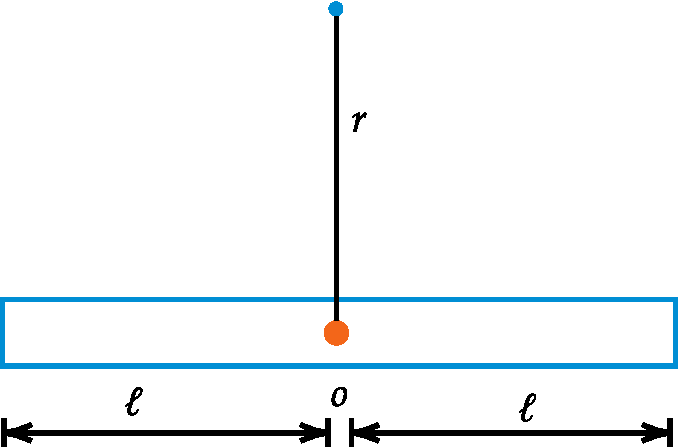
\includegraphics[width=0.25\textwidth]{electric field p2 ans}
		
\end{exercise}
\opencutright
\renewcommand\windowpagestuff{
	\centering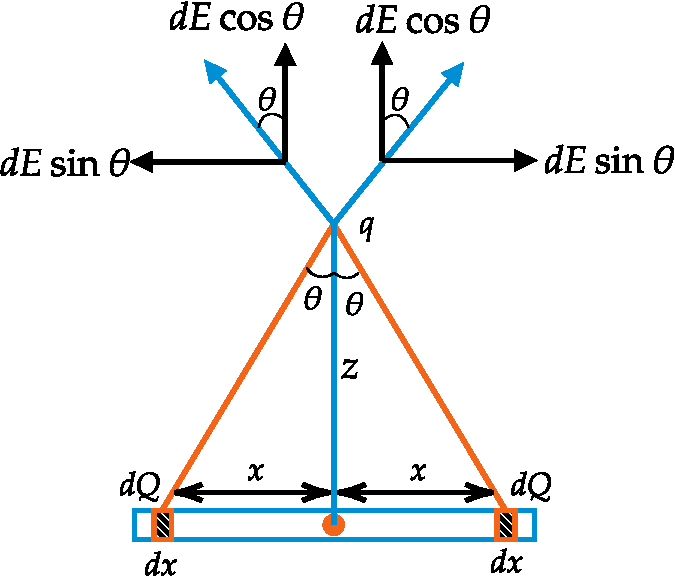
\includegraphics[width=5cm]{electric field p2}}
\begin{answer}
	\begin{cutout}{3}{\dimexpr\linewidth-4.9cm\relax}{2pt}{3}
		\begin{align*}
		\text{The elementary electric field}&\text{ at point $p$ due to $dQ$ is,}\\
		dE&=\frac{1}{4 \pi \epsilon_{0}} \frac{dQ}{(x^{2}+z^{2})}
			\end{align*}
		\end{cutout}
	On resolving the components of $dE$ both the x-components\\ cancells out only the y-components exist.Then,
	
	\begin{align*}
	dE_{y}&=2dE \cos\theta\\
	&=2\cdot\frac{1}{4 \pi \epsilon_{0}}\frac{z dQ}{(z^{2}+x^{2})^{3/2}}\hat{j}\\
	&=2\cdot\frac{1}{4 \pi \epsilon_{0}}\frac{z \lambda dx}{(r^{2}+x^{2})^{3/2}}\hat{j}\\
	E_{y}&=2\cdot\int_{0}^{\ell} \frac{1}{4 \pi \epsilon_{0}}\frac{z \lambda dx}{(z^{2}+x^{2})^{3/2}}\\
	&=2\cdot\left.\frac{ \lambda z}{4 \pi \varepsilon_{0}}\left[\frac{x}{z^{2} \sqrt{z^{2}+x^{2}}}\right]\right|_{0} ^{\ell}\\
	&=\frac{1}{4 \pi \varepsilon_{0}} \frac{2 \lambda \ell}{z \sqrt{z^{2}+\ell^{2}}} \hat{j}
	\end{align*}
\end{answer}

\subsubsection{Electric Field Lines}
An electric line of force is an imaginary curve drawn in such a way that tangent to this curve at any point gives the direction of electric field at the point.The strength of the field is indicated by the length of the arrow, whereas the spacing of the lines indicates the field strength
(with closer lines signifying a stronger field).Experimentally, the direction of the arrow is the direction in which a positive test charge would move when placed in the vicinity of the source.\\
\textbf{Properties} 
\begin{itemize}
	\item Electric field lines must originate on positive charge and terminate on negative charge.
	\item The net electric field at any point is the vector sum of all electric fields present at that point.
	\item Electric field lines can never cross, since that would indicate that the field points in two different directions at the same location (if two or more different sources contribute electric fields pointing in different directions at the same location, the total electric field is the vector sum of the individual fields, and the electric field lines always point in the
	single direction of the total field).
	\item Electric field lines are always perpendicular to the surface of a
	conductor in equilibrium.
\end{itemize}
The figures below shows the electric field of some charge distributions.
\begin{figure}[H]
	\begin{center}
		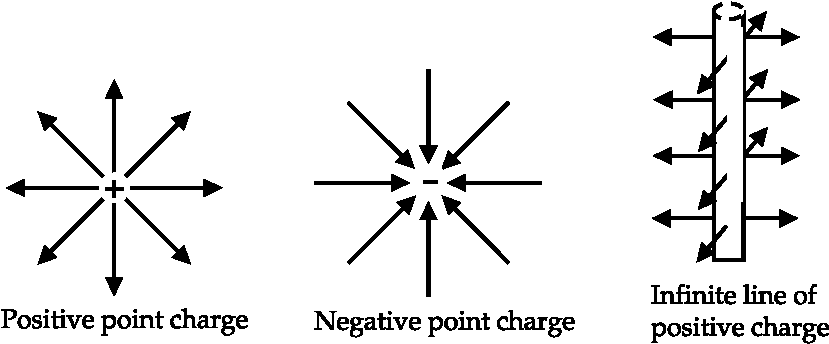
\includegraphics[width=0.60\textwidth]{electric field lines 1}
	\end{center}
	\begin{center}
		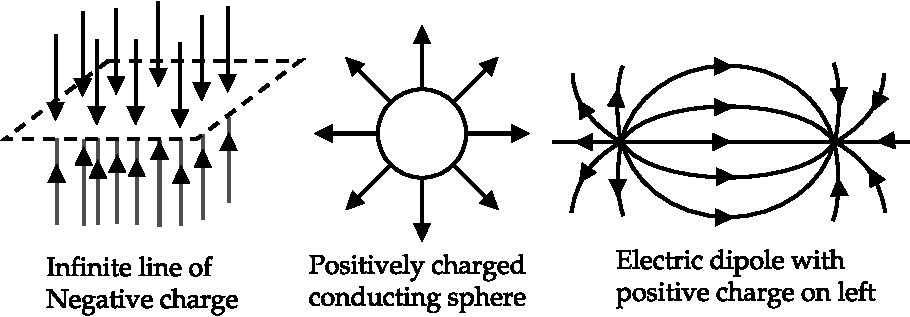
\includegraphics[width=0.60\textwidth]{electric field lines 2}
	\end{center}
\caption{Electric field lines due to different type of charge distributions.}
\end{figure}

\subsubsection{Electric Flux}
\begin{definition}
The flux of electric field $ \vec{E} $ through a surface $\vec{S}  $, is a measure of the “number of electric field lines” passing through that surface.\end{definition}
We know that an infinitesimal surface  can be looked upon as a vector with the magnitude equal to the area and the direction along the outward normal to the surface. In the figure \ref{Electric flux} we see electric field lines passing through a surface $\vec{S}$, the direction of the electric
field making an angle $\theta$ with the normal to the surface. Then the flux of the electric field is defined as, 
\begin{align}
\phi&=\int_{S} \vec{E} \cdot d \vec{S} \\
\phi&=\int_{S} {E} \cos \theta d {S}
\end{align} 

\begin{figure}[H]
	\begin{center}
		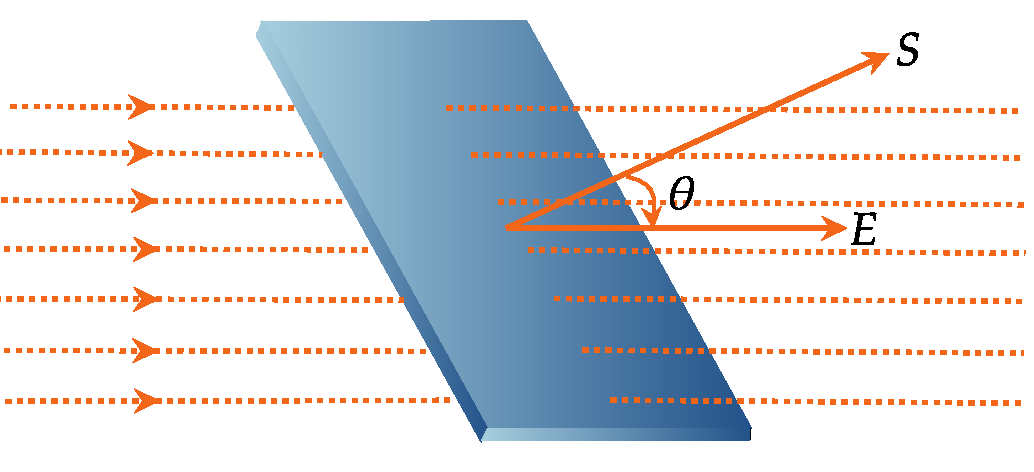
\includegraphics[width=0.50\textwidth]{Electricflux}
	\end{center}
	\caption{Electric Flux}
	\label{Electric flux}
\end{figure}
\subsection{Gauss' Law}
\begin{definition}
	According to Gauss' law, the total electric flux through any closed surface is equal to $\frac{1}{\varepsilon_{0}}$ times the total charge enclosed by the surface.
	For a closed surface $ 'S' $ enclosing $n$ number of point charges $q_{1} \ldots \ldots q$, the mathematical formula is
	$$\oint \vec{E} \cdot d \vec{S}=\frac{1}{\varepsilon_{0}} \sum_{i=1}^{n} q_{i}$$
\end{definition}
\subsubsection{Proof}
Suppose a point charge $q$ located at $O$ and we consider a closed surface enclosing $q$. Let us consider an elementary area $d \vec{S}=\hat{n} d s$ at distance $r$ from $O$ Therefore, the electric field at $P$ is,\\
\begin{minipage}{0.70\textwidth}
	$$
	\vec{E}=\frac{1}{4 \pi \varepsilon_{0}} \frac{q}{r^{2}} \hat{r}
	$$
	\\Therefore, the flux through the $d \vec{S}$ is
\begin{align*}
\vec{E} \cdot d \vec{S}&=\frac{1}{4 \pi \varepsilon_{0}} \frac{q}{r^{2}} \hat{r} \hat{n} d s\\
\text{Therefore, total flux} &=\oint \vec{E} \cdot d \vec{s}\\
	&=\frac{q}{4 \pi \varepsilon_{0}} \oint \frac{\hat{r} \cdot \hat{n}}{r^{2}} d S\\ 
	&=\frac{q}{4 \pi \varepsilon_{0}} \oint \frac{d S \cos \theta}{r^{2}} \rightarrow\oint \frac{d S \cos \theta}{r^{2}}=\text{solid angle} =4\pi\\
	&=\frac{q}{4 \pi \varepsilon_{0}} 4 \pi=\frac{q}{\varepsilon_{0}}\\
	\vec{E} \cdot d \vec{S}&=\frac{q_{enclosed}}{\varepsilon_{0}}
\end{align*}
\end{minipage}
\begin{minipage}{0.30\textwidth}
\begin{figure}[H]
	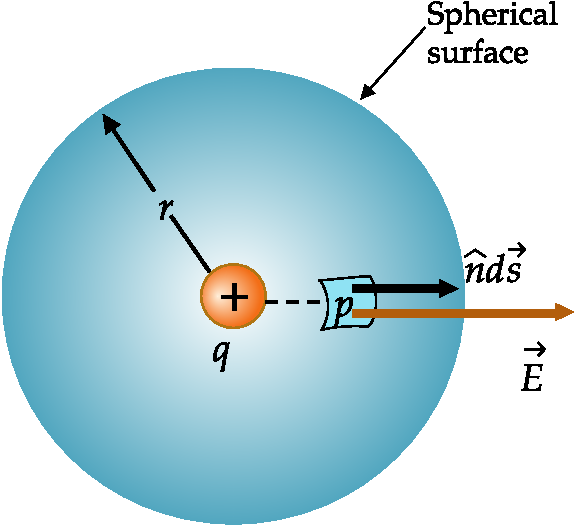
\includegraphics[width=0.95\textwidth]{gausslaw}
	\caption{Gauss law.}
\end{figure}
\end{minipage}
\begin{note}
	Suppose, instead, the charge $ q $ is somewhere outside the volume.  If we draw electric field lines from the charge on to the volume,  they will intersect the surface at two places.Every field lines entering the surface will leave out and the total flux adds up to zero. Any surface, whether real or imaginary, through which flux of an electric field  is calculated is called a “Gaussian surface”
\end{note}

\begin{figure}[H]
	\begin{center}
		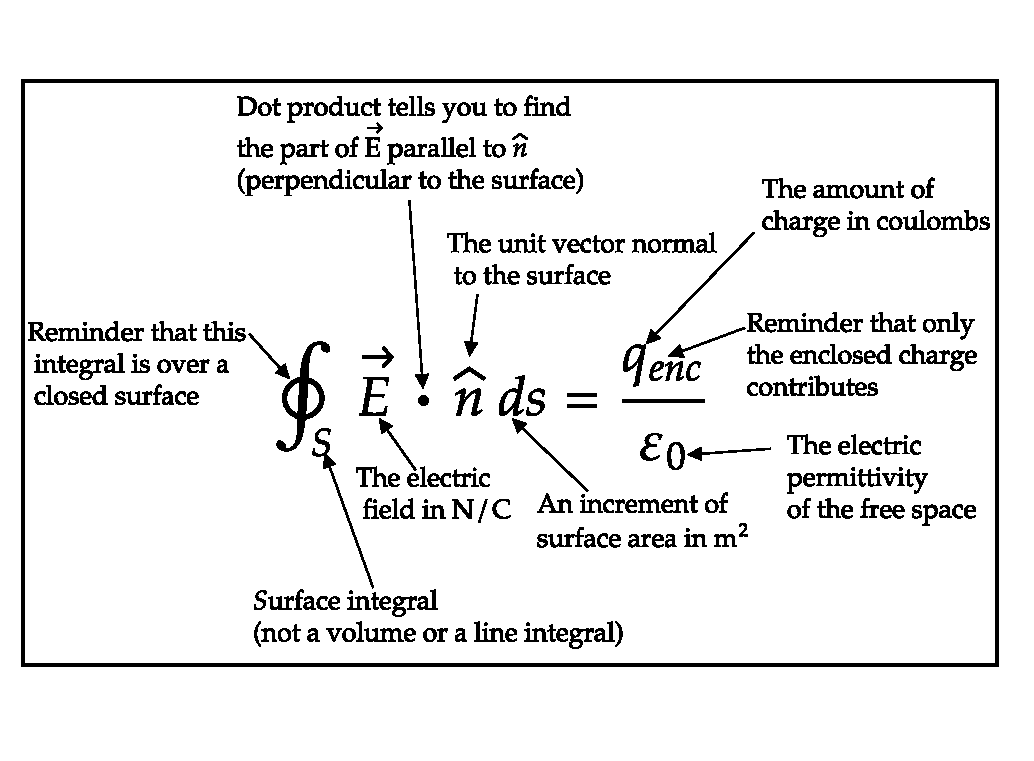
\includegraphics[width=0.75\textwidth]{gauss law 1}
	\end{center}
\end{figure}

\subsubsection{Differential Form of Gauss Laws}
We know that Gauss's law is,
$$
\oint \vec{E} \cdot d \vec{S}=\frac{q}{\varepsilon_{0}}
$$
For continuous change distribution
\begin{alignat*}{2}
& \oint \vec{E} \cdot d \vec{S}&&=\int \frac{\rho d v}{\varepsilon_{0}} \\
\Rightarrow & \int(\vec{\nabla} \cdot \vec{E}) d v&&=\int \frac{\rho d v}{\varepsilon_{0}} \\
& \vec{\nabla} \cdot \vec{E}&&=\frac{\rho}{\varepsilon_{0}}
\end{alignat*}

This equation is the differential form of Gauss's law.
\begin{center}
\framebox{
	\parbox[t][2.5cm]{4cm}{
		
		\addvspace{0.2cm} \centering 
		\underline{\textbf{Gauss' Law}}\\\vspace{0.5cm}
$\oint \vec{E} \cdot d \vec{s}=\frac{q}{\varepsilon_{0}}$\\
$\vec{\nabla} \cdot \vec{E}=\frac{\rho}{\varepsilon_{0}}$	} }
\end{center}
\subsection{Application of Gauss Law in Field Calculation}
\subsubsection{Uniformly Charged Spherical Shell}
Consider a uniformly charged spherical shell having radius $\mathrm{R}$ and total charge $\mathrm{Q}$. To calculate electric field Let us draw spherical Gaussian surfaces by dotted lines in figure.\\ Due to symmetry to electric field lines are in radial direction.
\\
\begin{minipage}{0.75\textwidth}
	According to Gauss law,
\begin{align*}
\oint \vec{E} \cdot d \vec{S}&=\frac{Q_{\text {enclosed }}}{\varepsilon_{0}}\\
\oint E \hat{r} \cdot d S \hat{r}&=\frac{Q_{\text {enclosed }}}{\varepsilon_{0}}\\
\oint E d S&=\frac{Q_{\text {enclosed }}}{\varepsilon_{0}}\\
\text { Since all points on Gaussian sphere}&\text{ are at equal distance from center. Therefore. }\\
E \oint d S&=\frac{Q_{\text {enclosed }}}{\varepsilon_{0}} \\
E 4 \pi r^{2}&=\frac{Q_{\text {enclosed }}}{\varepsilon_{0}} \\
E&=\frac{Q_{\text {enclosed }}}{4 \pi \varepsilon_{0} r^{2}}\\
Q_{\text {enclosed }}&=0 \text { for } R<R, \quad E=0 \\
Q_{\text {enclosed }}&=Q \text { for } r>R=E=\frac{Q}{4 \pi \varepsilon_{0} r^{2}}
\end{align*}
Thus a sphere behaves like a point charge for outside point.
\end{minipage}
\begin{minipage}{0.25\textwidth}
	\begin{figure}[H]
		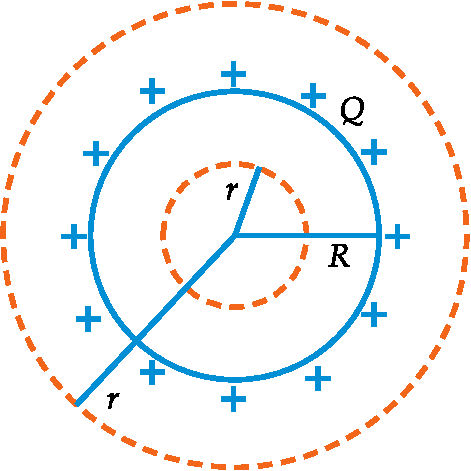
\includegraphics[width=0.95\textwidth]{holowsphere}
		\caption{Uniformly charged Spherical shell}
	\end{figure}
\end{minipage}


\subsubsection{Uniformly Charged Solid Sphere}
Consider uniformly charged sphere of radius $\mathrm{R}$ and total charge $\mathrm{Q}$,
\\Volume charge density, $\rho=\frac{Q}{\frac{4}{3} \pi R^{3}}=$ Constant
\\To calculate electric field draw Gaussian surfaces as shown by dotted lines in figure \\\begin{minipage}{0.75\textwidth}
	\begin{align*}
	E \oint d S&=\frac{Q_{\text {enclosed }}}{\varepsilon_{0}} \\
	E&=\frac{Q_{\text {enclosed }}}{4 \pi \varepsilon_{0} r^{2}}\\
	\text { for } r<R \quad Q_{\text {enc }}&=\int \rho d \tau=\rho \int_{0}^{r} d \tau=\rho \frac{4}{3} \pi r^{3} \\
	\therefore \quad E&=\frac{\rho r}{3 \varepsilon_{0}}=\frac{Q r}{4 \pi \varepsilon_{0} R^{3}} \\
	\text { for } r>R \quad Q_{\text {enc }}&=\int \rho d \tau=\rho \int_{0}^{R} d \tau=\rho \cdot \frac{4}{3} \pi R^{3} \\
	\therefore \quad E&=\frac{\rho R^{3}}{3 \varepsilon_{0} r^{2}}=\frac{Q}{4 \pi \varepsilon_{0} r^{2}} \quad \text { (same as point charge) }
\end{align*}
\end{minipage}
\begin{minipage}{0.25\textwidth}
	\begin{figure}[H]
		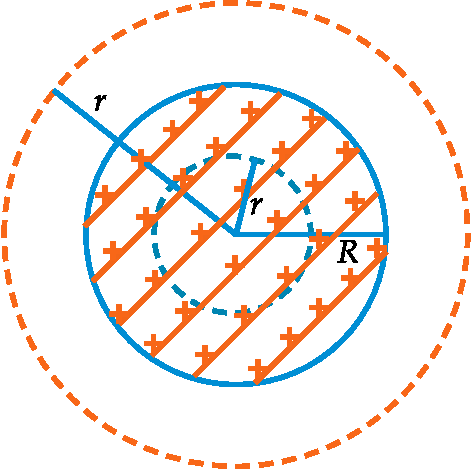
\includegraphics[width=0.95\textwidth]{solidsphere}
		\caption{Uniformly charged Solid sphere}
	\end{figure}
\end{minipage}
\subsubsection{Uniformly Charged Hollow Cylinder}
Consider a long hollow cylinder of radius $R$ and surface charge density $\sigma$ To calculate electric field let us draw cylindrical Gaussian surfaces as shown in the figure In this type cases electric field can be calculated only near the mid region because in the mid region field lines are in radial direction .\\
\begin{minipage}{0.75\textwidth}
\begin{align*}
\text{ According to Gauss' Law}\\
\oint \vec{E} \cdot d \vec{S}&=\frac{Q_{\text {enclosed }}}{\varepsilon_{0}}\\
\text{Here flux through flat surfaces}&\text{  of cylinder is zero}\\
\therefore \int_\text{curved} \vec{E} \hat{r} \cdot d S \hat{r}&=\frac{Q_{\text {enclosed }}}{\varepsilon_{0}}\\
\int_{\text {curved }} E d S&=\frac{Q_{\text {enclosed }}}{\varepsilon_{0}} \\
E \int dS&=\frac{Q_{\text {enclosed }}}{\varepsilon_{0}} \\
E \cdot 2 \pi r h&=\frac{Q_{\text {enclosed }}}{\varepsilon_{0}} \Rightarrow  E=\frac{Q_{\text {enc }}}{2 \pi \varepsilon_{0} r h}\\
\text{For}\quad r<R \quad Q_{\text {enclosed }}&=0, \quad E=0\\
\text{For}\quad r>R \quad Q_{\text {enclosel }}&=\sigma 2 \pi R h\\
\therefore \quad E&=\frac{\sigma R}{\varepsilon_{0} r}
\end{align*}
\end{minipage}
\begin{minipage}{0.25\textwidth}\hfil
	\begin{figure}[H]
		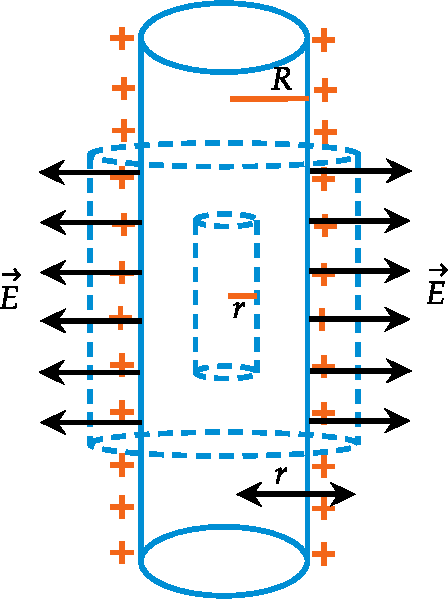
\includegraphics[width=0.95\textwidth]{hollowcylinder}
		\caption{Uniformly charged hollow cylinder}
	\end{figure}
\end{minipage}
\subsubsection{Uniformly Charged Solid Cylinder}
Consider a long solid cylinder of radius $R$ and surface charge density $\sigma$ To calculate electric field let us draw cylindrical Gaussian surfaces as shown in the figure,\\
\begin{minipage}{0.75\textwidth}
	\begin{align*}
	\text{ According to Gauss' Law}\\
	\oint \vec{E} \cdot d \vec{S}&=\frac{Q_{\text {enctosed }}}{\varepsilon_{0}}\\
	\text{Here flux through flat surfaces}&\text{  of cylinder is zero}\\
	\therefore \int_{curved} \vec{E} \hat{r} \cdot d S\hat{r}&=\frac{Q_{\text {cnclosed }}}{\varepsilon_{0}}\\
	E \int d S&=\frac{Q_{\text {enclosed }}}{\varepsilon_{0}} \\
	E&=\frac{Q_{\text {enclosed }}}{2 \pi \varepsilon_{0} r h}\\
	\text{For} \quad r<R \quad Q_{\text {enclosed }}&=\int_{0}^{r} \rho d \tau=\rho \int_{0}^{r} d \tau\\
	\therefore \quad Q_{\text {enclosed }}&=\rho \pi r^{2} h \\
	\therefore \quad E&=\frac{\rho r}{2 \varepsilon_{0}}\\
	\text{For }\quad r>R
	\quad Q_{\text {enclosed }}&=\int \rho d \tau=\rho \int d \tau=\rho \pi R^{2} h\\
	\therefore
	E&=\frac{\rho R^{2}}{2 \varepsilon_{0} r}
	\end{align*}
\end{minipage}
\begin{minipage}{0.25\textwidth}\hfil
	\begin{figure}[H]
		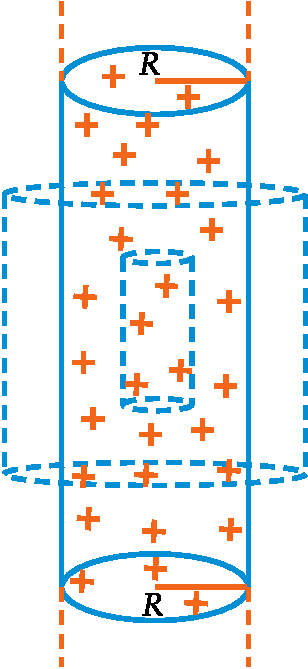
\includegraphics[width=0.70\textwidth]{solidcylinder}
		\caption{Uniformly charged solid cylinder}
	\end{figure}
\end{minipage}
\subsubsection{Uniformly Charged sheet(Non-Conducting)}
Consider a large sheet of surface charge density $\sigma$. Since the sheet is non conducting we assume that charge is only on one layer. To calculate electric field draw a cylindrical Gaussian surface as shown in the figure. Due to symmetry, field near the center of sheet is perpendicular to the sheet.\\
\begin{minipage}{0.75\textwidth}
	\begin{align*}
	\text { Gauss, law } \oint \vec{E} \cdot d \vec{S}&=\frac{Q_{\text {enclosed }}}{\varepsilon_{0}}\\
	\text{Flux is only through the flate surface}&\text{ of cylindrical Gaussian surface}\\
	\oint_{flat} \vec{E} \cdot d \vec{S}&=\frac{Q_{\text {enclosed }}}{\varepsilon_{0}}\\
	2 E A&=\frac{\sigma A}{\varepsilon_{0}} \cdot\\ \text { Therefore, } E&=\frac{\sigma}{2 \varepsilon_{0}}
	\end{align*}
\end{minipage}
\begin{minipage}{0.25\textwidth}\hfil
	\begin{figure}[H]
		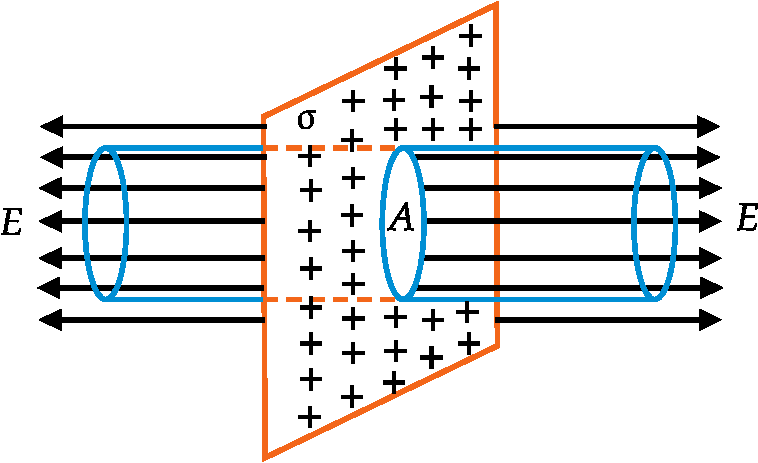
\includegraphics[width=1\textwidth]{chrgedsheet}
		\caption{Uniformly charged sheet}
	\end{figure}
\end{minipage}
\textbf{Conducting sheet :}\\ In conducting sheet charge resides on both sides therefore each layer gives a field $\sigma / 2 \varepsilon_{0}$.
Therefore, net field due to conducting sheet is $$E=\frac{\sigma}{\varepsilon_{0}}$$.
\begin{exercise}
	 A charge $q$ sits at the corner of a cube as shown in figure. What is the flux of $\vec{E}$ through one side?
	 \begin{figure}[H]
	 	\begin{center}
	 		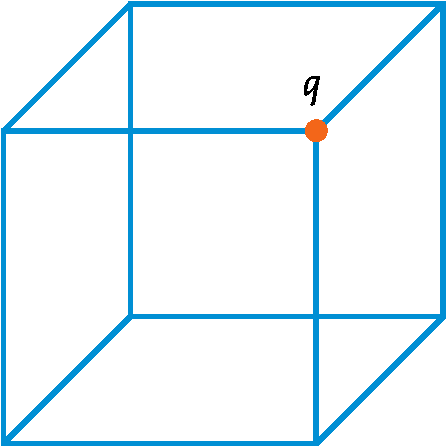
\includegraphics[width=0.10\textwidth]{gausss law2}
	 	\end{center}
	 \end{figure}
\end{exercise}
\begin{answer}
	Let consider a Gaussian surface in shape of cube whose sides are $2 a$.Now charge is at the centre.
	\begin{align*}
	\therefore  \text{Flux through the area}\ 24 a^{2} &= \frac{q}{\varepsilon_{0}}\\
	\therefore \text{Flux through the area}\ a^{2} &= \int_{\text {one face }} \vec{E} \cdot d \vec{a}\\&=\frac{1}{24} \int_{\text { whole  cube }} \vec{E} \cdot d \vec{S}\\&=\frac{q}{24 \varepsilon_{0}}
	\end{align*}
	
	
\end{answer}
\newpage
\begin{abox}
	Practice Set-1
\end{abox}
\begin{enumerate}[label=\color{ocre}\textbf{\arabic*.}]
	\item Consider two point charges $q$ and $\lambda q$ located at the points, $x=a$ and $x=\mu a$,
	respectively. Assuming that the sum of the two charges is constant, what is the value of
	$\lambda$ for which the magnitude of the electrostatic force is maximum?
	{\exyear{JEST 2015}}
	\begin{tasks}(4)
		\task[\textbf{A.}]  $\mu$
		\task[\textbf{B.}]1
		\task[\textbf{C.}]$\frac{1}{\mu}$
		\task[\textbf{D.}] $1+\mu$
	\end{tasks}
	\begin{answer}
		\begin{align*}
		F&=\frac{1}{4 \pi \varepsilon_{0}} \frac{(\lambda q \times q)}{(\mu a-a)^{2}}\\&=\frac{1}{4 \pi \varepsilon_{0}} \frac{\lambda q^{2}}{a^{2}(\mu-1)^{2}}\\&=\frac{1}{4 \pi \varepsilon_{0} a^{2}(\mu-1)^{2}} \frac{\lambda c^{2}}{(1+\lambda)^{2}} \quad \because q+\lambda q=c \\
		\text { For maximum } F, \frac{d F}{d \lambda}=0 \\0&= \frac{1}{4 \pi \varepsilon_{0} a^{2}(\mu-1)^{2}}\left[\frac{(1+\lambda)^{2} c^{2}-\lambda c^{2} \times 2(1+\lambda)}{(1+\lambda)^{4}}\right] \\
		\Rightarrow(1+\lambda)^{2} c^{2}&=\lambda c^{2} \times 2(1+\lambda)\\ \Rightarrow 1+\lambda&=2 \lambda \\\Rightarrow \lambda&=1
		\end{align*}
		Correct option is (B)
	\end{answer}
\item  An electric field in a region is given by $\vec{E}(x, y, z)=a x \hat{i}+c z \hat{j}+6 b y \hat{k} .$ For which values of
$a, b, c$ does this represent an electrostatic field?
{\exyear{JEST 2012}}

\begin{tasks}(4)
\task[\textbf{A.}]$13,1,12$ 
\task[\textbf{B.}]$17,6,1$
\task[\textbf{C.}]$13,1,6$
\task[\textbf{D.}]$45,6,1$
\end{tasks}
\begin{answer}
\begin{align*}
\intertext{ For electrostatic field,} 
\vec{\nabla} \times \vec{E}&=0\\
\vec{\nabla} \times \vec{E}&=\left[\begin{array}{ccc}
\hat{i} & \hat{j} & \hat{k} \\
\frac{\partial}{\partial x} & \frac{\partial}{\partial y} & \frac{\partial}{\partial z} \\
a x & c z & 6 b y
\end{array}\right]=0\\ \Rightarrow \vec{\nabla} \times \vec{E}&=(6 b-c) \hat{i}+\hat{j}[0-0]+\hat{k}[0]=0 \\
\Rightarrow(6 b-c) \hat{i}&=0 \\\Rightarrow c&=6 b
\end{align*}
Correct option is (C)
\end{answer}
% Question related to Image charge. 
%\question A point charge $+q$ is placed at $(0,0, d)$ above a grounded infinite conducting plane
%defined by $z=0$. There are no charges present anywhere else. What is the magnitude of
%electric field at $(0,0,-d)$ ?
%{\exyear{JEST 2012}}
%\begin{tasks}(4)
%\task[\textbf{A.}]  $\frac{q}{8\pi \in_{0} d^{2}}$
%\task[\textbf{B.}] $-\infty$
%\task[\textbf{C.}]0
%\task[\textbf{D.}]$\frac{q}{16 \pi \in_{0} d^{2}}$
%\end{tasks}
%\begin{answer}
%\begin{align*}
%\intertext{ Electric field at $Q$}
%\vec{E}&=\frac{-q}{4 \pi \epsilon_{0}(2 d)^{2}}(\hat{z})\\&=\frac{-q}{16 \pi \in_{0} d^{2}} \hat{z} \\\Rightarrow|E|&=\frac{q}{16 \pi \in_{0} d^{2}}
%\end{align*}
%Correct option is (D)
%\end{answer}
\item The electric fields outside $(r>R)$ and inside $(r<R)$ a solid sphere with a uniform
volume charge density are given by $\vec{E}_{r>R}=\frac{1}{4 \pi \varepsilon_{0}} \frac{q}{r^{2}} \hat{r}$ and $\vec{E}_{r<R}=\frac{1}{4 \pi \varepsilon_{0}} \frac{q}{R^{3}} r \hat{r}$
respectively, while the electric field outside a spherical shell with a uniform surface
charge density is given by $\vec{E}_{r>R}=\frac{1}{4 \pi \varepsilon_{0}} \frac{q}{r^{2}} \hat{r}, q$ being the total charge. The correct ratio of
the electrostatic energies for the second case to the first case is
{\exyear{JEST 2013}}
\begin{tasks}(4)
\task[\textbf{A.}] $1: 3$
\task[\textbf{B.}]$9: 16$
\task[\textbf{C.}]$3: 8$
\task[\textbf{D.}]$5: 6$
\end{tasks}
\begin{answer}
\begin{align*}
\intertext { Electrostatic energy in spherical shell ,}
w_{s p}&=\frac{\epsilon_{0}}{2} \int_{0}^{R}\left|\vec{E}_{1}\right|^{2} 4 \pi r^{2} d r+\frac{\epsilon_{0}}{2} \int_{R}^{\infty}\left|\vec{E}_{2}\right|^{2} 4 \pi r^{2} d r\\
\Rightarrow \frac{\epsilon_{0}}{2} \int_{R}^{\infty} \frac{q^{2}}{\left(4 \pi \in_{0}\right)^{2} r^{4}} 4 \pi r^{2} d r&=\frac{q^{2}}{8 \pi \in_{0}}\left(-\frac{1}{r}\right)_{R}^{\infty}\\&=\frac{q^{2}}{8 \pi \in_{0}} \frac{1}{R}
\intertext{Electrostatic energy in solid sphere,}
w_{s}&=\frac{\epsilon_{0}}{2} \int_{0}^{R}\left|E_{1}\right|^{2} 4 \pi r^{2} d r+\frac{\epsilon_{0}}{2} \int_{R}^{\infty}\left|E_{2}\right|^{2} 4 \pi r^{2} d r\\
\Rightarrow \frac{q^{2}}{8 \pi \in_{0}}& \times \frac{1}{R^{6}}\left[\frac{r^{5}}{5}\right]_{0}^{R}+\frac{q^{2}}{8 \pi \in_{0}}\left[-\frac{1}{r}\right]_{R}^{\infty}\\
w_{s}&=\frac{q^{2}}{5 \times 8 \pi \in_{0}} \cdot \frac{1}{R}+\frac{q^{2}}{8 \pi \in_{0} R}=\frac{6 q^{2}}{40 \pi \in_{0} R}\\
\text { Now }\ \frac{W_{\text {spherical }}}{W_{\text {sphere }}}&=\frac{\frac{q^{2}}{8 \pi \in_{0}R}}{\frac{6 q^{2}}{40 \pi \in_{0} R}}\\&=\frac{5}{6}
\end{align*}
Correct option is (D)
\end{answer}
\item  If $\vec{E}_{1}=x y \hat{i}+2 y z \hat{j}+3 x z \hat{k}$ and $\vec{E}_{2}=y^{2} \hat{i}+\left(2 x y+z^{2}\right) \hat{j}+2 y z \hat{k}$ then
{\exyear{JEST 2013}}
\begin{tasks}(1)
\task[\textbf{A.}]  Both are impossible electrostatic fields.
\task[\textbf{B.}]Both are possible electrostatic fields.
\task[\textbf{C.}]Only $\vec{E}_{1}$ is a possible electrostatic field.
\task[\textbf{D.}]Only $\vec{E}_{2}$ is a possible electrostatic field.
\end{tasks}
\begin{answer}
\begin{align*}
\text { For electrostatic field } \vec{\nabla} \times \vec{E}=0\\
\vec{\nabla} \times \vec{E}_{2}&=\left|\begin{array}{ccc}
\hat{i} & \hat{j} & \hat{k} \\
\frac{\partial}{\partial x} & \frac{\partial}{\partial y} & \frac{\partial}{\partial z} \\
y^{2} & 2 x y+z^{2} & 2 y z
\end{array}\right|=
(2 z-2 z) \hat{i}+0+(2 y-2 y) \hat{z}=0\\
\vec{\nabla} \times \vec{E}_{1}&=\left|\begin{array}{ccc}
\hat{i} & \hat{j} & \hat{k} \\
\frac{\partial}{\partial x} & \frac{\partial}{\partial y} & \frac{\partial}{\partial z} \\
x y & 2 y z & 3 x z
\end{array}\right|=(0-2 y) \hat{i}+0+x \hat{j} \neq 0
\end{align*}
Correct option is (D)
\end{answer}
\item A charge $q$ is placed at the centre of an otherwise neutral dielectric sphere of radius $a$
and relative permittivity $\varepsilon_{r} .$ We denote the expression $q / 4 \pi \varepsilon_{0} r^{2}$ by $E(r)$. Which of the
following statements is false?
{\exyear{JEST 2013}}
\begin{tasks}(1)
\task[\textbf{A.}] The electric field inside the sphere, $r<a$, is given by $E(r) / \varepsilon_{r}$
\task[\textbf{B.}] The field outside the sphere, $r>a$, is given by $E(r)$
\task[\textbf{C.}]The total charge inside a sphere of radius $r>a$ is given by $q$.
\task[\textbf{D.}]The total charge inside a sphere of radius $r<a$ is given by $q$. 
\end{tasks}
\begin{answer}
Correct option is (D)
\end{answer}
\item Two large nonconducting sheets one with a fixed uniform positive charge and another
with a fixed uniform negative charge are placed at a distance of 1 meter from each other.
The magnitude of the surface charge densities are $\sigma_{+}=6.8 \mu \mathrm{C} / \mathrm{m}^{2}$ for the positively
charged sheet and $\sigma_{-}=4.3 \mu \mathrm{C} / \mathrm{m}^{2}$ for the negatively charged sheet. What is the electric
field in the region between the sheets?
{\exyear{JEST 2014}}
\begin{tasks}(4)
\task[\textbf{A.}] $6.30 \times 10^{5} \mathrm{~N} / \mathrm{C}$
\task[\textbf{B.}]$3.84 \times 10^{5} \mathrm{~N} / \mathrm{C}$
\task[\textbf{C.}] $1.40 \times 10^{5} \mathrm{~N} / \mathrm{C}$
\task[\textbf{D.}] $1.16 \times 10^{5} \mathrm{~N} / \mathrm{C}$ 
\end{tasks}
\begin{answer}
\begin{align*}
\text { Electric field between the sheet is }&=\frac{\sigma_{+}}{2 \epsilon_{0}}+\frac{\sigma_{-}}{2 \epsilon_{0}}\\&=\frac{6.8 \times 10^{-6}}{2 \epsilon_{0}}+\frac{4.3 \times 10^{-6}}{2 \epsilon_{0}}\\
\frac{11.2 \times 10^{-6}}{2 \times 8.86 \times 10^{-12}}&=0.626 \times 10^{6} \Rightarrow 6.3 \times 10^{5} \mathrm{~N} / \mathrm{C}
\end{align*}
Correct option is (A)
\end{answer}
\item A circular loop of radius $R$, carries a uniform line charge density $\lambda$. The electric field,
calculated at a distance $z$ directly above the center of the loop, is maximum if $z$ is equal
to,
{\exyear{JEST 2015}}
\begin{tasks}(4)
\task[\textbf{A.}] $\frac{R}{\sqrt{3}}$
\task[\textbf{B.}] $\frac{R}{\sqrt{2}}$
\task[\textbf{C.}]$\frac{R}{2}$
\task[\textbf{D.}]$2 R$ 
\end{tasks}
\begin{answer}
\begin{align*}
E&=\frac{1}{4 \pi \varepsilon_{0}} \frac{(\lambda \times 2 \pi R) z}{\left(R^{2}+z^{2}\right)^{3 / 2}} \\
\text { For maximum } E,\  \frac{d E}{d z}&=0 \\\Rightarrow \frac{\lambda \times 2 \pi R}{4 \pi \varepsilon_{0}}\left[\frac{\left(R^{2}+z^{2}\right)^{3 / 2}-z \times 3 / 2 \sqrt{R^{2}+z^{2}} \times 2 z}{\left(R^{2}+z^{2}\right)^{3}}\right]&=0 \\
\Rightarrow\left(R^{2}+z^{2}\right)^{3 / 2}&=3 z^{2} \sqrt{R^{2}+z^{2}}\\ \Rightarrow R^{2}+z^{2}&=3 z^{2}\\ \Rightarrow R^{2}&=2 z^{2}\\ \Rightarrow z&=\frac{R}{\sqrt{2}}
\end{align*}
Correct option is (B)
\end{answer}
\end{enumerate}
\newpage
\begin{abox}
	Practise Set-2
\end{abox}
\begin{enumerate}[label=\color{ocre}\textbf{\arabic*.}]
\item Four equal point charges are kept fixed at the four vertices of a square. How many neutral points (i.e. points where the electric field vanishes) will be found inside the square?
{\exyear{NET/JRF(DEC-2011)}}
\begin{tasks}(4)
	\task[\textbf{A.}] 1
	\task[\textbf{B.}] 4
	\task[\textbf{C.}] 5
	\task[\textbf{D.}] 7
\end{tasks}
\begin{answer}
	\begin{align*}
	\intertext{Inside the square, there is only one point where field vanishes}
	\end{align*}
	So the correct answer is \textbf{Option (A)}
\end{answer}
\question A static charge distribution gives rise to an electric field of the form $\vec{E}=\alpha\left(1-e^{-r / R}\right) \frac{\hat{r}}{r^{2}}$, where $\alpha$ and $R$ are positive constants. The charge contained within a sphere of radius $R$, centred at the origin is
{\exyear{NET/JRF(DEC-2011)}}
\begin{tasks}(4)
	\task[\textbf{A.}] $\pi \alpha \varepsilon_{0} \frac{e}{R^{2}}$
	\task[\textbf{B.}]  $\pi \alpha \varepsilon_{0} \frac{e^{2}}{R^{2}}$
	\task[\textbf{C.}] $4 \pi \alpha \varepsilon_{0} \frac{R}{e}$
	\task[\textbf{D.}] $\pi \alpha \varepsilon_{0} \frac{R^{2}}{e}$
\end{tasks}
\begin{answer}
	\begin{align*}
	Q_{e n c}&=\varepsilon_{0} \oint \vec{E} \cdot d \vec{a}\\&=\alpha \varepsilon_{0} \int\left(1-e^{-r / R}\right) \frac{\hat{r}}{r^{2}} \cdot\left(r^{2} \sin \theta d \theta d \phi \hat{r}\right)\\&=\alpha \varepsilon_{0} \times \int_{0}^{\pi} \int_{0}^{2 \pi}\left(1-e^{-r / R}\right) \sin \theta d \theta d \phi\\
	\text{at }r&=R, \quad Q_{e n c}=4 \pi \alpha \varepsilon_{0}\left(1-\frac{1}{e}\right).\text{ So none of the options given are correct.}
	\end{align*}
	None of the options given are correct
\end{answer}
	\question Charges $Q, Q$ and $-2 Q$ are placed on the vertices of an equilateral triangle $A B C$ of sides of length $a$, as shown in the figure. The dipole moment of this configuration of charges, irrespective of the choice of origin, is
{\exyear{NET/JRF(JUNE-2012)}}

\begin{figure}[H]
\centering
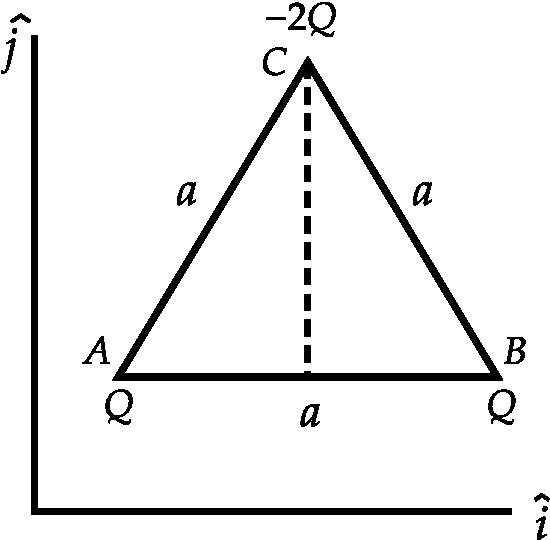
\includegraphics[height=4.5cm,width=4cm]{diagram-20211011(16)-crop}
\caption{}
\label{}
\end{figure}
\begin{tasks}(4)
\task[\textbf{A.}] $+2 a Q \hat{i}$
\task[\textbf{B.}] $+\sqrt{3} a Q \hat{j}$
\task[\textbf{C.}] $-\sqrt{3} a Q \hat{j}$
\task[\textbf{D.}] 0
\end{tasks}
\begin{answer}
\begin{align*}
\intertext{Let coordinates of $A$ is $(l, m)$, then}
\vec{p}&=q_{i} \vec{r}_{i}^{\prime}=Q[l \hat{i}+m \hat{j}]+Q[(l+a) \hat{i}+m \hat{j}]-2 Q\left[\left(l+\frac{a}{2}\right) \hat{i}+\left(m+\frac{\sqrt{3} a}{2}\right) \hat{j}\right]\\
\vec{p}&=Q[\hat{i}+m \hat{j}]+Q[(l+a) \hat{i}+m \hat{j}]-Q[(2 l+a) \hat{i}+(2 m+\sqrt{3} a) \hat{j}\rfloor \Rightarrow \vec{p}=-\sqrt{3} a Q \hat{j}
\end{align*}
So the correct answer is \textbf{Option (C)}
\end{answer}
 Three charges are located on the circumference of a circle of radius $R$ as shown in the figure below. The two charges $Q$ subtend an angle $90^{\circ}$ at the centre of the circle. The charge $q$ is symmetrically placed with respect to the charges $Q$. If the electric field at the centre of the circle is zero, what is the magnitude of $Q$ ?
{\exyear{NET/JRF(DEC-2012)}}

\begin{figure}[H]
\centering
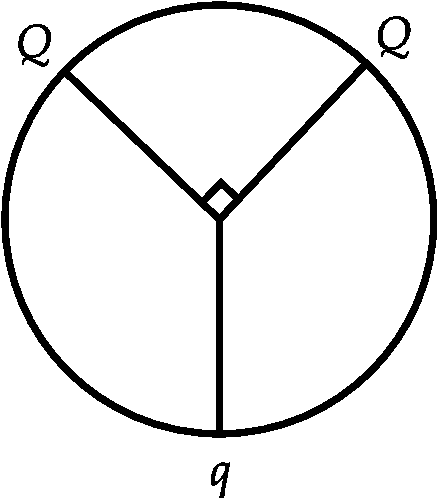
\includegraphics[height=4.5cm,width=4cm]{diagram-20211011(17)-crop}
\end{figure}
\begin{tasks}(4)
\task[\textbf{A.}] $q / \sqrt{2}$
\task[\textbf{B.}] $\sqrt{2} q$
\task[\textbf{C.}] $2 q$
\task[\textbf{D.}] $4 q$
\end{tasks}
\begin{answer}
\begin{align*}
E_{1}&=E_{2}=\frac{1}{4 \pi \varepsilon_{0}} \frac{Q}{R^{2}}\text{ and }E_{3}=\frac{1}{4 \pi \varepsilon_{0}} \frac{q}{R^{2}}\\
\text{Resultant of }E_{1}\text{ and }E_{2}\text{ is }E&=\sqrt{E_{1}^{2}+E_{2}^{2}}=\sqrt{2} E_{1},\\\text{ Thus }E_{3}&=E \Rightarrow Q=\frac{q}{\sqrt{2}}
\end{align*}
So the correct answer is \textbf{Option (A)}
\end{answer}
\item  A point charges $q$ of mass $m$ is kept at a distance $d$ below a grounded infinite conducting sheet which lies in the $x y$ - plane. For what value of $d$ will the charge remains stationary?
{\exyear{NET/JRF(DEC-2012)}}

\begin{tasks}(2)
\task[\textbf{A.}] $q / 4 \sqrt{m g \pi \varepsilon_{0}}$
\task[\textbf{B.}] $q / \sqrt{m g \pi \varepsilon_{0}}$
\task[\textbf{C.}] There is no finite value of $d$
\task[\textbf{D.}]  $\sqrt{m g \pi \varepsilon_{0}} / q$
\end{tasks}
\begin{answer}
There is attractive force between point charge $q$ and grounded conducting sheet that can be calculate from method of images i.e. $\frac{1}{4 \pi \varepsilon_{0}} \frac{q^{2}}{(2 d)^{2}}=m g \Rightarrow d=\frac{q}{4 \sqrt{m g \pi \varepsilon_{0}}}$\\
So the correct answer is \textbf{Option (A)}
\end{answer}
\item A solid sphere of radius $R$ has a charge density, given by
$$
\rho(r)=\rho_{0}\left(1-\frac{a r}{R}\right)
$$
where $r$ is the radial coordinate and $\rho_{0}, a$ and $R$ are positive constants. If the magnitude of the electric field at $r=R / 2$ is $1.25$ times that at $r=R$, then the value of $a$ is
{\exyear{NET/JRF(DEC-2014)}}

\begin{tasks}(4)
\task[\textbf{A.}] 2
\task[\textbf{B.}] 1
\task[\textbf{C.}]  $1 / 2$
\task[\textbf{D.}] $1 / 4$
\end{tasks}
\begin{answer}
\begin{align*}
\oint_{S} \vec{E} \cdot d \vec{a}&=\frac{1}{\varepsilon_{0}} Q_{e n c} \Rightarrow|\vec{E}| \times 4 \pi r^{2}=\frac{1}{\varepsilon_{0}} \int_{0}^{r} \rho_{0}\left(1-\frac{a r}{R}\right) 4 \pi r^{2} d r\\
\Rightarrow|\vec{E}| \times 4 \pi r^{2}&=\frac{4 \pi \rho_{0}}{\varepsilon_{0}} \int_{0}^{r}\left(r^{2}-\frac{a r^{3}}{R}\right) d r\\&=\frac{4 \pi \rho_{0}}{\varepsilon_{0}}\left(\frac{r^{3}}{3}-\frac{a r^{4}}{4 R}\right) \Rightarrow|\vec{E}|=\frac{\rho_{0}}{\varepsilon_{0}}\left(\frac{r}{3}-\frac{a r^{2}}{4 R}\right)\\
\because E_{r=R / 2}&=1.25 E_{r=R} \Rightarrow \frac{\rho_{0}}{\varepsilon_{0}}\left(\frac{R / 2}{3}-\frac{a R^{2} / 4}{4 R}\right)=1.25 \frac{\rho_{0}}{\varepsilon_{0}}\left(\frac{R}{3}-\frac{a R^{2}}{4 R}\right)\\
\Rightarrow\left(\frac{1}{6}-\frac{a}{16}\right)&=\frac{5}{4}\left(\frac{1}{3}-\frac{a}{4}\right) \Rightarrow\left(\frac{1}{6}-\frac{a}{16}\right)\\&=\left(\frac{5}{12}-\frac{5 a}{16}\right) \Rightarrow \frac{5 a}{16}-\frac{a}{16}=\frac{5}{12}-\frac{1}{6}\\
\Rightarrow \frac{4 a}{16}&=\frac{5-2}{12} \Rightarrow \frac{a}{4}=\frac{3}{12} \Rightarrow a=1
\end{align*}
So the correct answer is \textbf{Option (B)}
\end{answer}
	\item Consider a charge $Q$ at the origin of 3 - dimensional coordinate system. The flux of the electric field through the curved surface of a cone that has a height $h$ and a circular base of radius $R$ (as shown in the figure) is
{\exyear{NET/JRF(DEC-2015)}}

\begin{figure}[H]
\centering
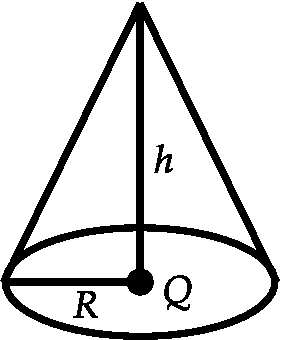
\includegraphics[height=3cm,width=2.5cm]{diagram-20211011(36)-crop}
\end{figure}
\begin{tasks}(4)
\task[\textbf{A.}] $\frac{Q}{\epsilon_{0}}$
\task[\textbf{B.}] $\frac{Q}{2 \epsilon_{0}}$
\task[\textbf{C.}] $\frac{h Q}{R \in_{0}}$
\task[\textbf{D.}] $\frac{Q R}{2 h \in_{0}}$
\end{tasks}
\begin{answer}
So the correct answer is \textbf{Option (B)}
\end{answer}
\item Four equal charges of $+Q$, each are kept at the vertices of a square of side $R$. A particle of mass $m$ and charge $+Q$ is placed in the plane of the square at a short distance $a(\ll R)$ from the centre. If the motion of the particle is confined to the plane, it will undergo small oscillations with an angular frequency
{\exyear{NET/JRF(JUNE-2016)}}

\begin{tasks}(4)
\task[\textbf{A.}] $\sqrt{\frac{Q^{2}}{2 \pi \varepsilon_{0} R^{3} m}}$
\task[\textbf{B.}] $\sqrt{\frac{Q^{2}}{\pi \varepsilon_{0} R^{3} m}}$
\task[\textbf{C.}] $\sqrt{\frac{\sqrt{2} Q^{2}}{\pi \varepsilon_{0} R^{3} m}}$
\task[\textbf{D.}] $\sqrt{\frac{Q^{2}}{4 \pi \varepsilon_{0} R^{3} m}}$
\end{tasks}
\begin{answer}$\left. \right. $
\begin{figure}[H]
	\centering
	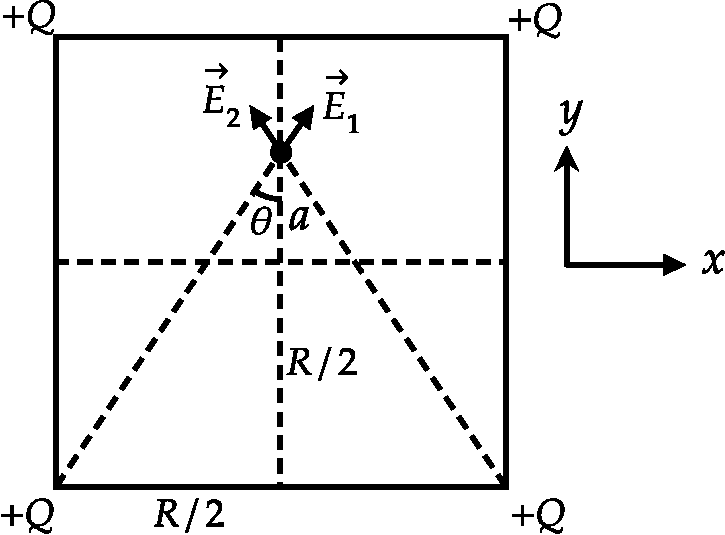
\includegraphics[height=5cm,width=7cm]{diagram-20211011(39)-crop}
\end{figure}
\begin{align*}
E_{1}&=E_{2}=\frac{k Q}{\left[\left(a+\frac{R}{2}\right)^{2}+\frac{R^{2}}{4}\right]}\\
\text{Resultant field }E_{12, y}&=2 E_{1} \cos \theta\\
E_{12, y}&=\frac{2 k Q}{\left[\left(a+\frac{R}{2}\right)^{2}+\frac{R^{2}}{4}\right]^{\frac{3}{2}}}\left(a+\frac{R}{2}\right) \approx \frac{2 k Q}{\left[\frac{R^{2}}{2}\right]^{\frac{3}{2}}}\left(a+\frac{R}{2}\right)\\
E_{12, y}&=\frac{4 \sqrt{2} k Q}{R^{3}}\left(a+\frac{R}{2}\right)\\
\end{align*}
\begin{figure}[H]
	\centering
	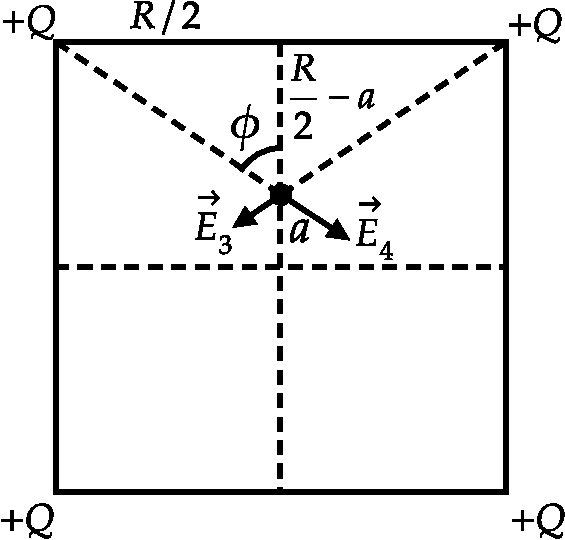
\includegraphics[height=5cm,width=5.5cm]{diagram-20211011(40)-crop}
\end{figure}
\begin{align*}
\text{	Similarly; }E_{3}&=E_{4}=\frac{k Q}{\left[\left(\frac{R}{2}-a\right)^{2}+\frac{R^{2}}{4}\right]}\\
\text{Resultant }E_{34, y}&=2 E_{3} \cos \phi
=\frac{2 k Q}{\left[\left(\frac{R}{2}-a\right)^{2}+\frac{R^{2}}{4}\right]^{\frac{3}{2}}}\left(\frac{R}{2}-a\right)\\
\Rightarrow \quad E_{34, y}&=\frac{4 \sqrt{2} k Q}{R^{3}}\left(\frac{R}{2}-a\right)\\
\text{Resultant }E&=\frac{4 \sqrt{2} k Q}{R^{3}}\left[\left(\frac{R}{2}-a\right)-\left(\frac{R}{2}+a\right)\right]=-\frac{8 \sqrt{2} k Q}{R^{3}} a\\
E&=\frac{-8 \sqrt{2}}{R^{3}} \times \frac{1}{4 \pi \varepsilon_{0}} Q a \Rightarrow E=-\frac{2 \sqrt{2} Q}{\pi \varepsilon_{0} R^{3}} a\\
\Rightarrow \quad F&=Q E=-\frac{2 \sqrt{2} Q^{2}}{\pi \varepsilon_{0} R^{3}} a \Rightarrow \omega=\sqrt{\frac{2 \sqrt{2} Q^{2}}{\pi \varepsilon_{0} m R^{3}}}
\end{align*}
So the correct answer is \textbf{Option (C)}
\end{answer}
\item Consider a sphere $S_{1}$ of radius $R$ which carries a uniform charge of density $\rho$. A smaller sphere $S_{2}$ of radius $a<\frac{R}{2}$ is cut out and removed from it. The centres of the two spheres are separated by the vector $\vec{b}=\frac{\hat{n} R}{2}$, as shown in the figure. The electric field at a point $P$ inside $S_{2}$ is
{\exyear{NET/JRF(JUNE-2016)}}

\begin{figure}[H]
\centering
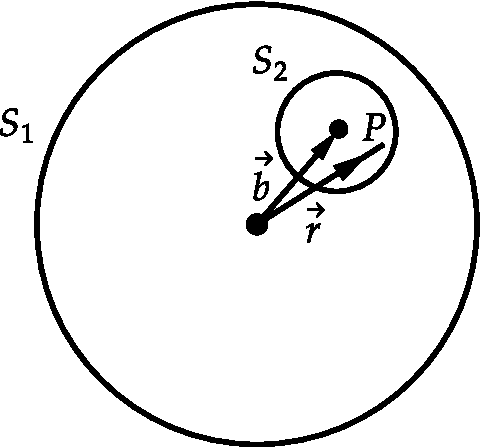
\includegraphics[height=4cm,width=4.2cm]{diagram-20211011(43)-crop}
\end{figure}
\begin{tasks}(4)
\task[\textbf{A.}]$\frac{\rho R}{3 \varepsilon_{0}} \hat{n}$
\task[\textbf{B.}] $\frac{\rho R}{3 \varepsilon_{0} a}(\vec{r}-\hat{n} a)$
\task[\textbf{C.}] $\frac{\rho R}{6 \varepsilon_{0}} \hat{n}$
\task[\textbf{D.}] $\frac{\rho a}{3 \varepsilon_{0} R} \vec{r}$ 
\end{tasks}
\begin{answer}$\left. \right. $
\begin{figure}[H]
	\centering
	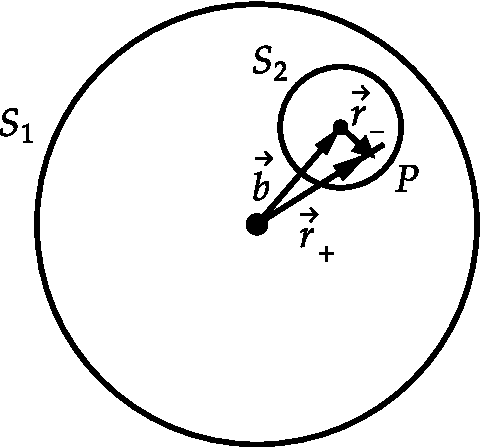
\includegraphics[height=4cm,width=4.2cm]{diagram-20211011(44)-crop}
\end{figure}
\begin{align*}
\text{Electric field at $P$ due to $S_{1}$ is }\vec{E}_{1}&=\frac{\rho}{3 \varepsilon_{0}} \vec{r}_{+}
\intertext{Electric field at $P$ due to $S_{2}$ (assume $\left.-\rho\right)$ is $\vec{E}_{2}=\frac{-\rho}{3 \varepsilon_{0}} \vec{r}_{-}$}
\text{Thus }\vec{E}&=\vec{E}_{1}+\vec{E}_{2}=\frac{\rho}{3 \varepsilon_{0}}\left(\vec{r}_{+}-\vec{r}_{-}\right) ; \\ \because \vec{b}+\vec{r}_{-}&=\vec{r}_{+} \Rightarrow \vec{r}_{+}-\vec{r}=\vec{b}\\
\vec{E}&=\frac{\rho}{3 \varepsilon_{0}} \vec{b}=\frac{\rho R}{6 \varepsilon_{0}} \hat{n}\left(\because \vec{b}=\frac{R}{2} \hat{n}\right)
\end{align*}
So the correct answer is \textbf{Option (C)}
\end{answer}
\item  The charge per unit length of a circular wire of radius $a$ in the $x y$-plane, with its centre at the origin, is $\lambda=\lambda_{0} \cos \theta$, where $\lambda_{0}$ is a constant and the angle $\theta$ is measured from the positive $x$-axis. The electric field at the centre of the circle is
{\exyear{NET/JRF(DEC-2016)}}

\begin{tasks}(4)
\task[\textbf{A.}] $\vec{E}=-\frac{\lambda_{0}}{4 \in_{0} \alpha} \hat{i}$
\task[\textbf{B.}] $\vec{E}=\frac{\lambda_{0}}{4 \in_{0} \alpha} \hat{i}$
\task[\textbf{C.}] $\vec{E}=-\frac{\lambda_{0}}{4 \in_{0} \alpha} \hat{j}$
\task[\textbf{D.}] $\vec{E}=\frac{\lambda_{0}}{4 \pi \in_{0} \alpha} \hat{k}$
\end{tasks}
\begin{answer}$\left. \right. $\\
\begin{figure}[H]
	\centering
	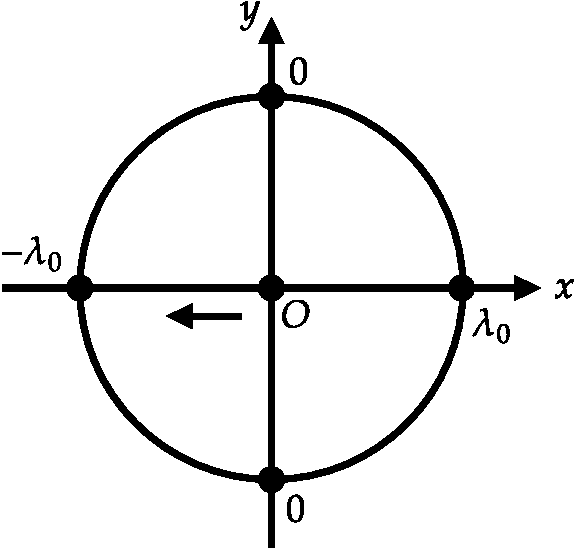
\includegraphics[height=4cm,width=4.1cm]{diagram-20211011(47)-crop}
\end{figure}
At centre $O$, direction of field is $-\hat{x}$.\\
So the correct answer is \textbf{Option (A)}
\end{answer}
\end{enumerate}


\newpage
\begin{abox}
	Practise Set-3
	\end{abox}
\begin{enumerate}[label=\color{ocre}\textbf{\arabic*.}]
\item Consider a point charge $+q$ revolving around another charge $+Q$ in a circular orbit. Find the angular velocity of in which $+q$ is rotating.
	\begin{figure}[H]
		\begin{center}
			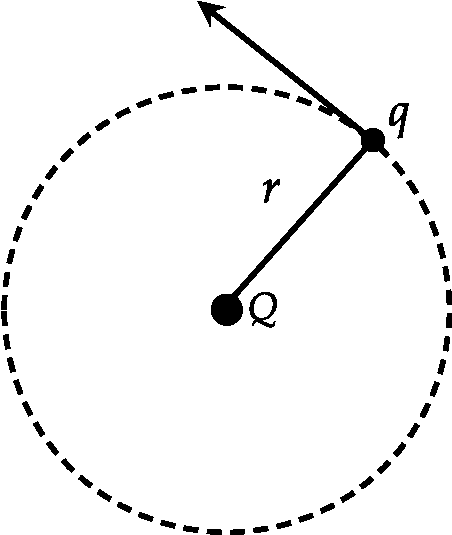
\includegraphics[width=0.15\textwidth]{pset3-1}
		\end{center}
	\end{figure}
	\begin{answer}
		Due to mutual repulsion of charges $q$ makes a circular motion around $Q$
		\begin{align*}
		\text{Necessary centripetal motion}&=\text{ Coulombic force}\\
		F_{centripetal}&=F_{coulombic}\\
		\frac{mV^{2}}{r}&=\frac{1}{4\pi \epsilon_{0}}\frac{Qq}{r^{2}}\\
		\frac{m{(r \omega)}^{2}}{r}&=\frac{1}{4\pi \epsilon_{0}}\frac{Qq}{r^{2}}\qquad \because V=r\omega\\
		\omega&=\sqrt{ \frac{1}{4\pi \epsilon_{0}}\frac{Qq}{mr^{3}}}
		\end{align*}
	\end{answer}
\item Two identical positive point charges $Q$ each are fixed at a distance $2 a$ apart. A point charge $q$ lies midway between the fixed charges. Show that
\begin{enumerate}
	\item For small displacement (relative to $a$ ) along line joining the fixed charges, the charge $q$ executes SHM if it is positive.
	\item For small lateral displacement, it executes SHM if it is negative. Compare the frequencies of oscillation in the two cases.
	\begin{answer}\hspace{0.5cm}
		\begin{enumerate}[label=(\alph*)]
			\item Let $x$ be the displacement of the charge $+q$ from the mean position. Now net force acting on the charge $q$ to bring in its original position.
			\begin{align*}
				F &=-\frac{Q q}{4 \pi \varepsilon_{0}(a-x)^{2}}+\frac{Q q}{4 \pi \varepsilon_{0}(a+x)^{2}} \\
				&=-\frac{Q q}{4 \pi \varepsilon_{0}} \frac{4 a x}{\left(a^{2}-x^{2}\right)^{2}} \approx-\frac{Q q}{4 \pi \varepsilon_{0}} \cdot \frac{4 a x}{a^{4}}=\frac{Q q}{4 \pi \varepsilon_{0}} \frac{4 x}{a^{3}}\\
				\text { Restoring force }&=F \frac{4 Q q}{4 \pi \varepsilon_{0} a^{3}} x=-K_{1} x, \text { (where, } m \text { is the mass of the charge) }
			\end{align*}
			As acceleration is directly proportional to displacement, hence the motion is SHM. Its time period $T_{1}$ is
			given by
			$$\omega_{1}=\sqrt{\frac{k_{1}}{m}}=\sqrt{\frac{4 Q q}{4 \pi \varepsilon_{0} m a^{3}}}$$
			\item Restoring force on $-q$ towards $Q$ is given by
			
			\begin{align*}
			F&=\frac{-2 Q q}{4 \pi \varepsilon_{0}\left(a^{2}+y^{2}\right)} \cdot \frac{y}{\left(a^{2}+y^{2}\right)}\\&=\frac{-2 Q q y}{4 \pi \varepsilon_{0}\left(a^{2}+y^{2}\right)^{3 / 2}} \approx \frac{-2 Q q y}{4 \pi \varepsilon_{0} a^{3}}\\&=-k_{2} y \\
			\omega_{2}&=\sqrt{\frac{k_{2}}{m}}\\&=\sqrt{\frac{2 Q q}{4 \pi \varepsilon_{0} m a^{3}}} \\\Rightarrow \frac{\omega_{1}}{\omega_{2}}&=\sqrt{2}
			\end{align*}
			
		\end{enumerate}
	\end{answer}
\end{enumerate}
\item Consider a fixed charge $Q$ and another point charge $q$ are placed at a seperation $r$ on a plane.Find the velocity of $q$ if it is mvng due to mutual repulsion.\begin{figure}[H]
	\begin{center}
		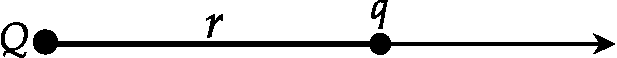
\includegraphics[width=0.35\textwidth]{pset3-3}
	\end{center}
\end{figure}
\begin{answer}
	\begin{align*}
	\text{Here, the coulombic force on}\quad q,F_{c}&=\frac{1}{4 \pi \varepsilon_{0}} \frac{Qq}{r^{2}}\\
	\text{We know that,}\quad F&=ma\\
	&=m\frac{dv}{dt}=m\frac{dv}{dx}\frac{dx}{dt}=m\frac{dv}{dx} v\\
	\text{Here,}\quad F_{c}&=F\\
	\frac{1}{4 \pi \varepsilon_{0}} \frac{Qq}{r^{2}}&=m\frac{dv}{dx} v\\
	\int_{0}^{v}v dv&=\frac{1}{4 \pi \varepsilon_{0}} \frac{Qq}{m} \int_{r_{1}}^{r_{2}}\frac{dr}{r^{2}}\\
	\left[ \frac{v^{2}}{2}\right] _{0}^{v}&=\frac{1}{4 \pi \varepsilon_{0}} \frac{Qq}{m} \left[ \frac{-1}{r}\right] _{r_{1}}^{r_{2}}\\
	\frac{v^{2}}{2}&=\frac{1}{4 \pi \varepsilon_{0}} \frac{Qq}{m}\left[ \frac{1}{r_{1}}-\frac{1}{r_{2}}\right] 
	\end{align*}

\end{answer}
\item Consider two identical pendulum of mass $m$ and charge $q$ are suspended from a support as shown . Due to mutual repulsion the charges are moving apart. Find the leakage of charge $\frac{dq}{dt}$.
\begin{answer} From the figure,\\
	\begin{figure}[H]
	\begin{minipage}{0.35\textwidth}
		
			\begin{center}
				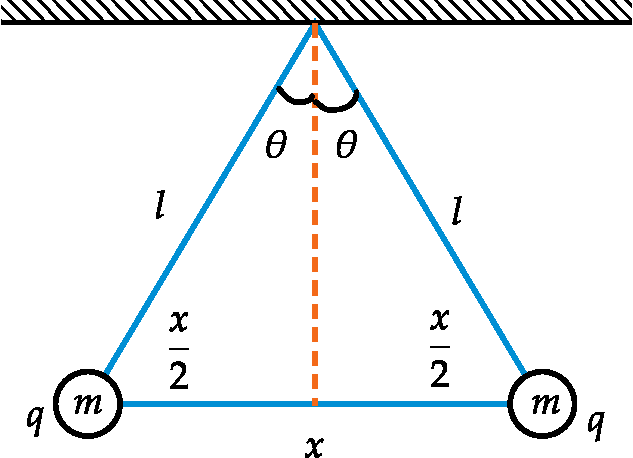
\includegraphics[width=0.85\textwidth]{pset3-4(1)}
			\end{center}
	\end{minipage}\hspace{2cm}
		\begin{minipage}{0.35\textwidth}	
		\begin{center}
			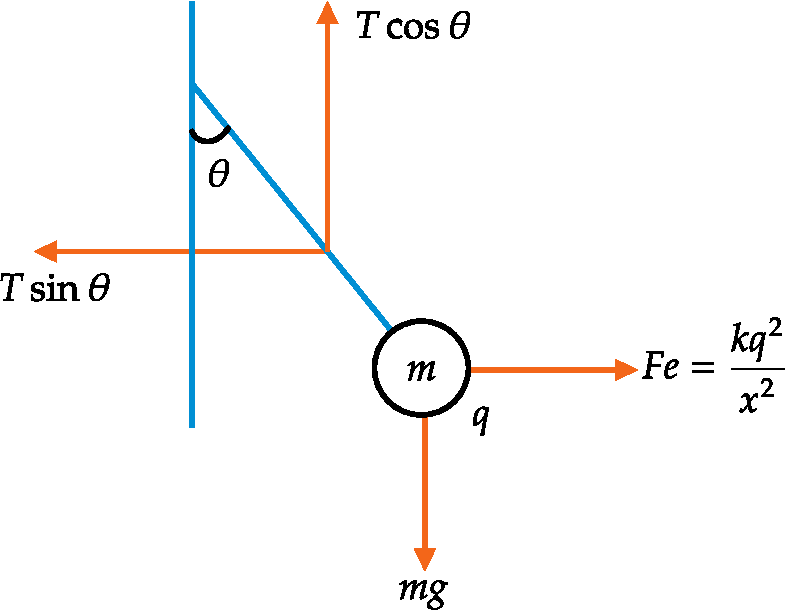
\includegraphics[width=0.85\textwidth]{pset3-4}
		\end{center}
	\end{minipage}
\end{figure}
	\begin{minipage}{0.35\textwidth}
	\begin{align*}
	\text{Here,} \tan \theta&=\frac{F_{e}}{mg}\\
	\frac{x}{2l}&=\frac{kq^{2}}{x^{2}mg}\\
	q^{2}&=\frac{x^{3}mg}{2kl}     \\
	q&=\left[\frac{mg}{2kl} \right]^{\frac{1}{2}} x^{\frac{3}{2}}\\
	\frac{dq}{dt}&=\frac{3}{2}\left[\frac{mg}{2kl} \right]^{\frac{1}{2}}  x^{\frac{1}{2}} \frac{dx}{dt}\\
	\frac{dq}{dt}&=\frac{3}{2}\left[\frac{mgx}{2kl} \right]^{\frac{1}{2}} v
	\end{align*}

\end{minipage}\hspace{2cm}
\begin{minipage}{0.35\textwidth}	
	
	\begin{align*}
	T\sin\theta&=F_{e}\\
	T\cos\theta&=mg\\
	\text{But, }\tan \theta&\approx\sin\theta\\
	\sin\theta&=\frac{x}{2l}
	\end{align*}
\end{minipage}
		

	
	


\end{answer}
\item A pendulum bob of mass $80 \mathrm{mg}$ and carrying a charge of $4 \times 10^{-8}$ coulomb is at rest in a horizontal uniform electric field of $20,000 \mathrm{Vm}^{-1}$. Find the tension in the thread of the pendulum and the angle it makes with the vertical (Take $g=10 \mathrm{~m} / \mathrm{s}^{2}$ )
\opencutright
\renewcommand\windowpagestuff{
	\centering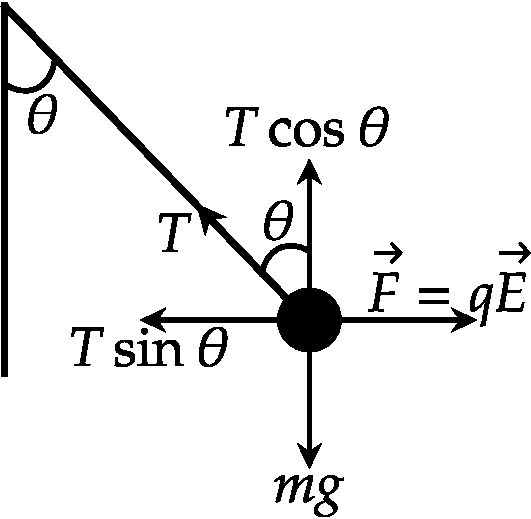
\includegraphics[width=3.5cm]{pset-3(6)}}
\begin{answer}
	The different forces on the bob are shown in figure :
	\begin{cutout}{2}{\dimexpr\linewidth-6cm\relax}{4pt}{3}
	\begin{align*}
	\text{Here,}\ m&=80 \mathrm{mg}=80 \times 10^{-6} \mathrm{~kg}\\
	q&=4 \times 10^{-8} \mathrm{C}\\
	{E}&=2 \times 10^{4} \mathrm{Vm}^{-1}
	\end{align*}
  \end{cutout}
	\begin{align*}
\text{Resolving} T,
\text{vertical component}&=T \cos \theta\\
\text{horizontal component}&=T \sin \theta
\end{align*}
	\begin{align}
\text{	For the equilibrium of the bob}\\
T \cos \theta&=m g \label{pset-3(6)}\\
\text { and } \quad T \sin \theta&=q E \label{pset-3(6-1)}
\end{align}
	Dividing eq.\ref{pset-3(6-1)} by \ref{pset-3(6)} we get,
\begin{align*}
\tan \theta&=\frac{q E}{m g}=\frac{4 \times 10^{-8} \times 2 \times 10^{4}}{80 \times 10^{-6} \times 10}\\&=1 \Rightarrow \theta=45^{\circ}\\
\text{Square and add equations}& \ref{pset-3(6-1)} \text{  and  } \ref{pset-3(6)},\text{ to get } T
\\T&=\sqrt{T ^{2}\cos^{2}\theta +T^{2} \sin^{2}\theta}\\
&=\sqrt{(m g)^{2}+(q E)^{2}} =
8 \sqrt{2} \times 10^{-4} N
\end{align*}
\end{answer}
\item A thin fixed ring of radius 1 metre has a positive charge $Q=1 \times 10^{-5}$ coulomb uniformly distributed over it. A particle of mass $m=0.9 \mathrm{gm}$ and having a negative charge of $q=1 \times 10^{-6}$ coulomb is placed on the axis at a distance of $1 \mathrm{~cm}$ from the centre of the ring. Show that the motion of the negatively charged particle is approximately simple harmonic. Calculate the time period of oscillations.

\opencutright
\renewcommand\windowpagestuff{
	\centering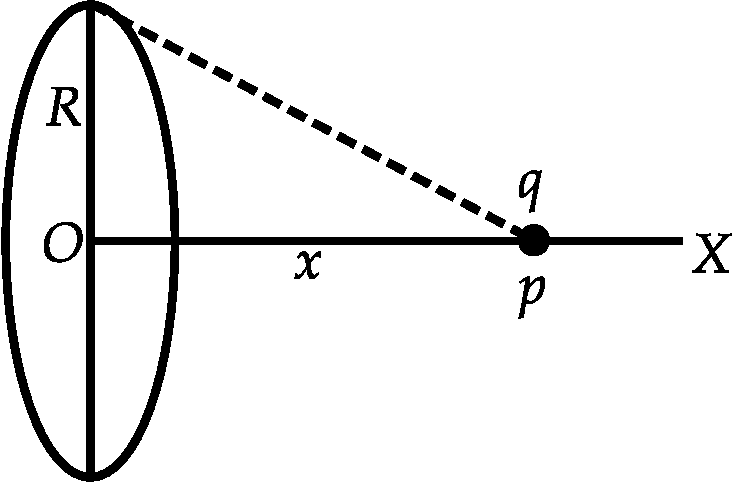
\includegraphics[width=4cm]{pset-2(6)}}
\begin{answer}
	Let the charge is placed at distance $x$ from center of ring as shown in figure: \\
	We know that field near center of ring is,
	\begin{cutout}{2}{\dimexpr\linewidth-6cm\relax}{4pt}{3}
	
	\begin{align*}
	E&=\frac{Q x}{4 \pi \varepsilon_{0} R^{3}}\\
	\text{Here,} x<<1
	\end{align*}
	Therefore, force on the point charge is	
	\end{cutout}
	\begin{align*}
	F=q E&=-\frac{q Q x}{4 \pi \varepsilon_{0} R^{3}}\\&=\frac{-1 \times 10^{-6} \times 10^{-5} \times 10^{9}}{1^{3}} x \\
	F&=-9 \times 10^{-2} x \\
	\quad F &\propto-x
	\end{align*}
	Therefore, motion is S.H.M. (comparing with $F=-k x$ )
	We get $k=9 \times 10^{-2}$\\
	\begin{align*}
		\text { Therefore, time period }&=2 \pi \sqrt{\frac{m}{k}}\\&=2 \pi \sqrt{\frac{0.9 \times 10^{-3}}{9 \times 10^{-2}}}\\&=\frac{2 \pi}{10}=\frac{\pi}{5}\text{ seconds}
	\end{align*}


\end{answer}
\item Four equal positive charges each of value $Q$ are fixed at the four corners of a square of side $a$. A unit positive charge mass $m$ is placed at $P$, at a height $h$ above the centre of the square. What should be the value of $Q$ in order that this unit charge is in equilibrium.
\begin{answer}
	Force experienced by unit positive charge placed at $P$ due to a charge $Q$ at $A$ is given by
	\begin{align*}
	F&=\frac{1}{4 \pi \varepsilon_{0}} \frac{Q \times 1}{\left(h^{2}+(\frac{a}{2})^{2}\right)}
	\end{align*}
	Since the magnitude of charge at $B, C$ and $D$ are equal,equal forces act on unit positive charge at $P$. When these forces are resolved in horizontal and vertical directions, the horizontal components $(F \cos \theta)$ cancel each other and the net vertical force is the sum of $\sin$ components .$4 F \sin \theta$.Then,
	\begin{align*}
	F_{total}&=4 \frac{1}{4 \pi \varepsilon_{0}} \frac{Q}{\left(h^{2}+\frac{a^{2}}{2}\right)} \cdot \sin \theta\\
	\text{For the equilibrium ,at $P$,}\\
	\text{Upward force}&=\text{Weight of unit charge}\\
	4 \frac{1}{4 \pi \varepsilon_{0}} \frac{Q}{\left(h^{2}+\frac{a^{2}}{4}\right)} \cdot \sin \theta&=m g\\
		\text { From figure, } \sin \theta&=\left\{\frac{h}{\sqrt{\left(h^{2}+a^{2} / 2\right)}}\right\} \\
	\therefore \frac{1}{\pi \varepsilon_{0}} \frac{Q h}{\left(h^{2}+\frac{a^{2}}{4}\right)^{3 / 2}}&=m g \\\text {  or } Q&=\frac{m g \pi \varepsilon_{0}}{h}\left(h^{2}+\frac{a^{2}}{4}\right)^{3 / 2}
	\end{align*}
	
	
\end{answer}
\item Consider a sphere of radius $R$ and spherical charge density,$\rho(r)= 
\begin{cases}
\frac{A}{r},& \text{for } r\leq R\\
0,              & \text{for }  r\geq R
\end{cases}$ Find the electric field ouside, inside and on the surface of the sphere.
\begin{answer}
	We need to find the total charge enclosed in the sphere,\begin{align*}
	q_{enc}&= \int \rho dv=\int_{0}^{R}\frac{A}{r} r^{2}dr\sin \theta d\theta d \phi\\
	&= A4\pi\int_{0}^{R} rdr =2\pi AR^{2} 	\text{ Then, }\\
   \underline{ E_{out}:}\\
    \oint_{S}\vec{E}\cdot \vec{S}&=\frac{q_{enc}}{\epsilon_{0}}\\
    E\cdot 4\pi r^{2}	&=\frac{2\pi AR^{2}}{\epsilon_{0}}\\
     E_{out}	&=\frac{ AR^{2}}{2\epsilon_{0}r^{2}}\\
     \underline{ E_{on}(r=R):}\\
     E_{on}	&=\frac{ AR^{2}}{2\epsilon_{0}R^{2}}\\
     &=\frac{ A}{2\epsilon_{0}}\\
     \underline{ E_{in}:}\\
     \oint_{S}\vec{E}\cdot \vec{S}&=\frac{q_{enc}}{\epsilon_{0}}\\
      E\cdot 4\pi r^{2}	&=\frac{2\pi Ar^{2}}{\epsilon_{0}}\\
      &=\frac{ A}{2\epsilon_{0}}
     \end{align*}
\end{answer}
\item Consider two solid spheres of opposite  charge densities, $+\rho \text{and } -\rho $ overlap each other.Find $\vec{E}$ in the overlap.
\begin{figure}[H]
	\begin{center}
		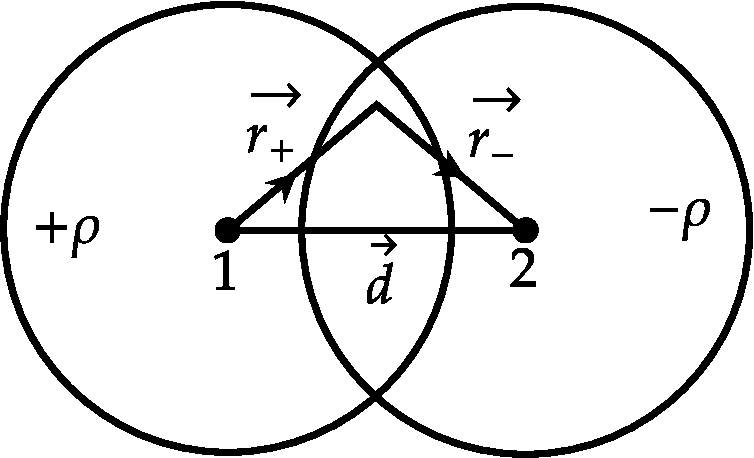
\includegraphics[width=0.25\textwidth]{pset-3(9)}
	\end{center}
\end{figure}
\begin{answer}
	From the figure,
	\begin{align*}
	\vec{d}+\vec{r_{-}}&=\vec{r_{+}}\\
	\vec{d}&=\vec{r_{+}}-\vec{r_{-}}\\
	E_{+}&=\frac{+\rho \vec r_{+}}{3\epsilon_{0}}\quad;\quad
	E_{-}=\frac{-\rho \vec r_{-}}{3\epsilon_{0}}\\
		E_{net}&=\frac{-\rho }{3\epsilon_{0}}(\vec r_{+}-\vec r_{-})=\frac{-\rho }{3\epsilon_{0}}\vec{d}
	\end{align*}
	Thus the electric field of the overlappping region only depends on the seperation between the spheres.
\end{answer}
\item Consider a particle of electric charge ' $e$ ' and mass ' $m$ ' moving under the influence of constant horizontal electric field $E$ and constant vertical gravitational field described by acceleration due to gravity ' $g$ '. If the particle starts from rest, what will be its trajectory? 

\begin{tasks}(4)
	\task[\textbf{a.}]Parabolic 
	\task[\textbf{b.}]Elliptic
	\task[\textbf{c.}]Straight line 
	\task[\textbf{d.}]Circular 
\end{tasks}

	\opencutright
	\renewcommand\windowpagestuff{
		\centering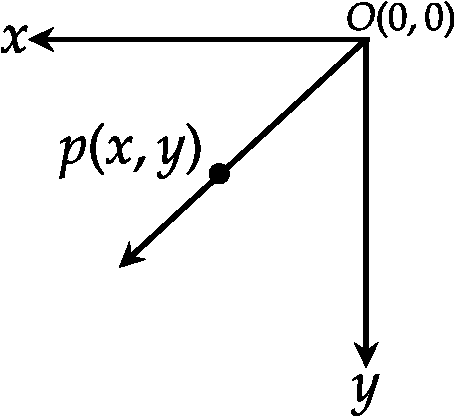
\includegraphics[width=3cm]{pset-3(10)}}
	\begin{answer}
	Let at $t=0$, electron at origine $(0,0)$ at $t=t$ the particle is at $(x, y)$.
		\begin{cutout}{3}{\dimexpr\linewidth-4cm\relax}{0pt}{3}
			\begin{align*}
		\text{Acceleration along $x$ -axis }&= \frac{e E}{m} \\ \text{acceleration along $y$ -axis}&= g\\
		\text{Therefore, the position of the}&\text{  particle at a time $t$ is,}\\ x=\frac{1}{2} \frac{e E}{m} t^{2}&\text{ and  } y=\frac{1}{2} g t^{2}\\
		\therefore  \frac{y}{x} &=\left(\frac{g m}{e E}\right) \\
		y&=\left(\frac{g m}{e E}\right) x\\
		\text{This is the equation of a straight line}
		\end{align*}
		\end{cutout}
		
	\end{answer}
\end{enumerate}
